\chapter{Casi d'uso}\label{chap:xenocase}

Questo Capitolo raccoglie tutti principali casi d'uso sviluppati per \Xeno. Con la dicitura `caso d'uso', ci si riferisce ad una tecnica usata nei processi di ingegneria del software, per effettuare in maniera esaustiva e non ambigua, la raccolta dei requisiti per produrre un software di qualit\`a e in linea con le specifiche richieste.

L'analisi dei casi d'uso verr\`a affrontata categorizzando gli argomenti della Web Application in macro funzionalit\`a. La suddivisione qui utilizzata corrisponde alle suddivisioni utilizzate per la creazione del menu di \Xeno, ovvero:
\begin{itemize}
	\item \textbf{caricamento xenopazienti} nel sistema;
	\item \textbf{aggiornamento dello status} di uno xenopaziente;
	\item \textbf{misurazioni}, divise in \textit{misurazioni qualitative} e \textit{misurazioni quantitative};
	\item gestione \textbf{impianti};
	\item gestione \textbf{espianti}.
\end{itemize}	

Nell'illustrare i vari casi d'uso, si proceder\`a illustrando i requisti delle varie aree, descrivendo l'interfaccia sviluppata e il flusso di dati che la caratterizza. Nella fase di sviluppo di queste interfacce, si \`e cercato di rimanere il pi\`u fedele possibile alle direttive iniziali, apportando il minor numero possibile di modifiche, in modo tale da soddisfare al meglio i bisogno dell'IRCC di Candiolo.

In Figura~\ref{fig:useCase} \`e riportato lo schema generale dei casi d'uso. All'interno di questo Capitolo, si analizzer\`a con maggior dettaglio ogni componente di questa figura.

\begin{figure}[h]
\begin{center}
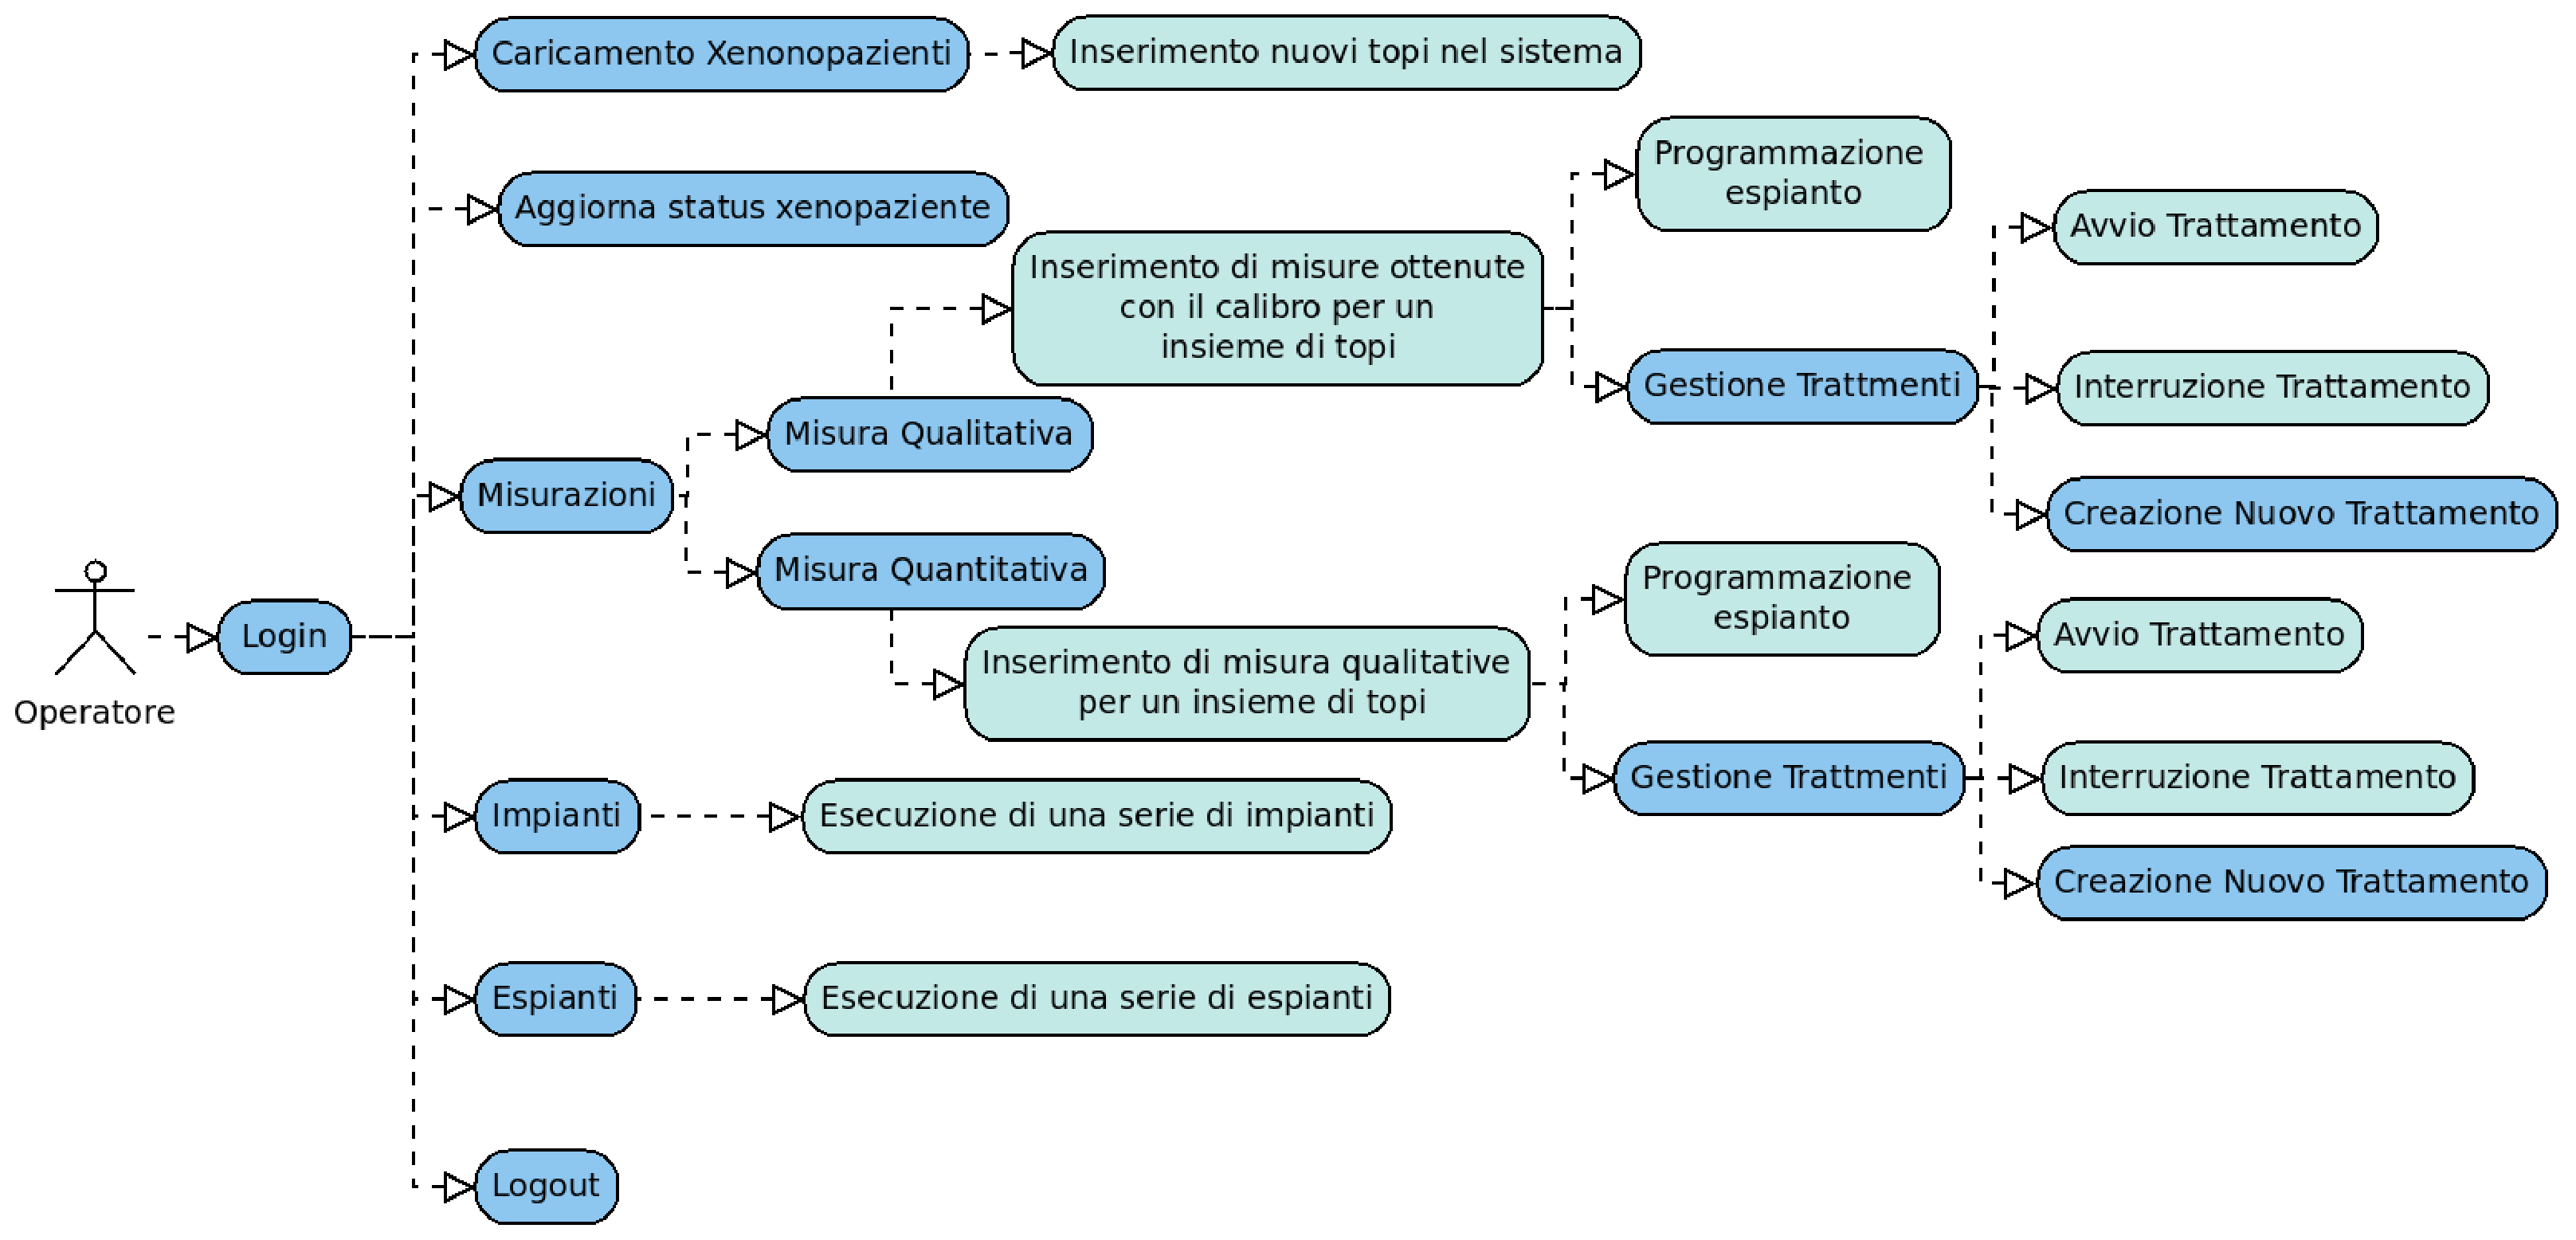
\includegraphics[width=1\textwidth]{./Figure/use_case}
\end{center}
\caption{Caso d'uso generico}\label{fig:useCase}
\end{figure}

\section{Caricamento xenopazienti nel sistema}

Questa interfaccia ha il compito di fornire all'operatore un metodo veloce ed intuitivo per immettere nel sistema i dati relativi a nuovi xenopazienti. In Figura~\ref{fig:UCDmiceL} \`e riportato il diagramma dei casi d'uso relativo a questa interfaccia.

\begin{figure}[h]
\begin{center}
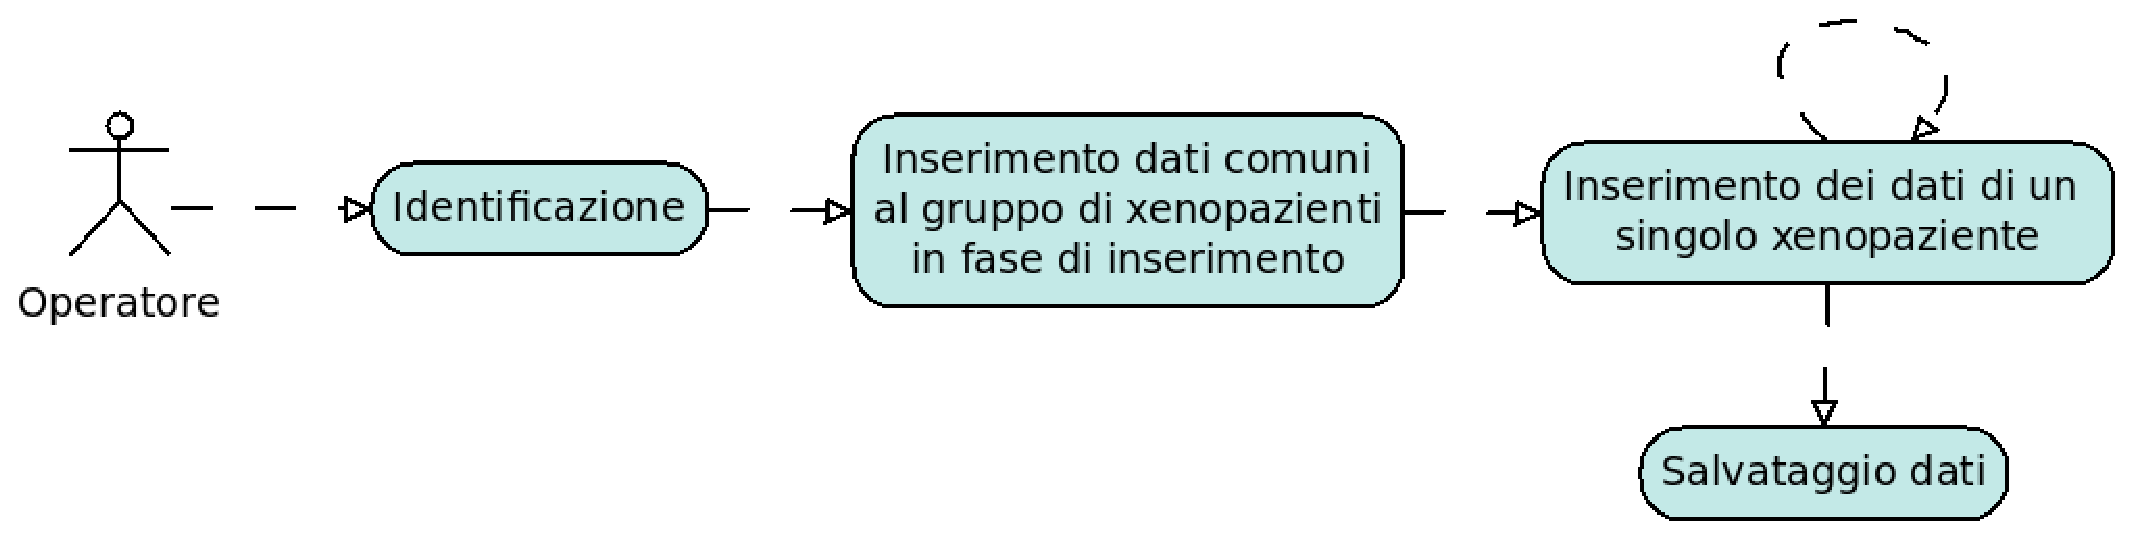
\includegraphics[width=0.7\textwidth]{./Figure/UCDmiceloading}
\end{center}
\caption{UCD del caricamento xenopazienti\label{fig:UCDmiceL}}
\end{figure}

Gli xenopazienti sono inseriti nel database in gruppi pi\`u o meno numerosi. Per snellire la procedura, all'operatore si presenta una schermata per immettere i dati comuni a tutti gli xenopazienti del gruppo. Questi dati comuni sono molteplici. Uno di questi \`e la data di disponibilit\`a, il cui valore di default \`e la data odierna, che indica la data dalla quale si possono utilizzare i topi ricevuti. Un altro parametro da inserire, molto importante, \`e lo status di partenza dei nuovi xenopazienti, selezionabile tramite un'apposita tendina. I dati proposti presenti in questa tendina sono presi dalla tabella Status del database. Inoltre, si inserisce anche l'et\`a presunta, in settimane, del carico di topi. Questa et\`a viene utilizzata per calcolare la data di nascita dei vari xenopazienti inseriti. Si inserisco anche il fornitore del carico di topi e il gruppo di ricerca al quale vengono assegnati.

Successivamente, si accede ad un'altra schermata, dove \`e possibile inserire i dati di ogni singolo topo. I dati necessari per ogni xenopaziente sono il suo barcode e il sesso di appartenenza. Si \`e quindi sviluppato un campo di testo per il barcode e due radio button, uno per i topi maschi e uno per i topi femmina. Il barcode pu\`o essere immesso da tastiera oppure attraverso l'utilizzo di un apposito lettore di microchip, leggendo il barcode in esso contenuto. \`E presente anche un tasto per confermare l'inserimento di un singolo xenopaziente, dopo averne inserito i dati. Effettuata l'immissione dellle informazioni relative ad un topo, queste vengono inserite in una lista, che mostra tutti gli xenopazienti inseriti fino a quel momento. Per velocizzare l'inserimento ed evitare di dover cliccare il bottone di conferma ad ogni topo, si \`e associato l'inserimento nella lista alla ricezione del carattere \textit{return} (invio). Questo particolare \`e molto importante per massimizzare i vantaggi derivanti dall'utilizzo del lettore di microchip. Infatti, si pu\`o associare il carattere return alla fine di ogni lettura di barcode, automatizzando cos\`i l'inserimento di uno xenopaziente con una singola operazione. In questo modo si conferisce maggior libert\`a all'operatore, il quale pu\`o effettuare le operazioni di immissione dati con maggiore velocit\`a.

Se si cercano di sottomettere dei dati errati (ad esempio una stringa in un campo riservato a numeri interi) o formatatti in modo scoretto (ad esempio, una data scritta non correttamente), i campi che li contengono vengono evidenziati da un messaggio che descrive il tipo di errore riscontrato, aiutando l'utente ad inserire i dati in maniera corretta.

Per rimediare ad eventuali errori nell'immissione dati (ad esempio, si inserisce il sesso sbagliato), si pu\`o utilizzare la funzione di cancellazione all'interna del la lista degli xenopazienti gi\`a inseriti. Questa lista ha infatti sia una funzione di riepilogo dinamico, sia la possibilit\`a di cancellare, uno ad uno, gli inserimenti gi\`a effettuati, prima dell'effettivo salvataggio nel database.

Una volta terminato, si inviano i dati al server, il quale li elabora e fornisce un report dei dati salvati, a meno che non si sia verificato un errore del sistema. In Figura~\ref{fig:SDmiceL} \`e riportato il diagramma delle sequenze di questa interfaccia, che riepiloga i vari passi descritti in precedenza.

\begin{figure}[h]
\begin{center}
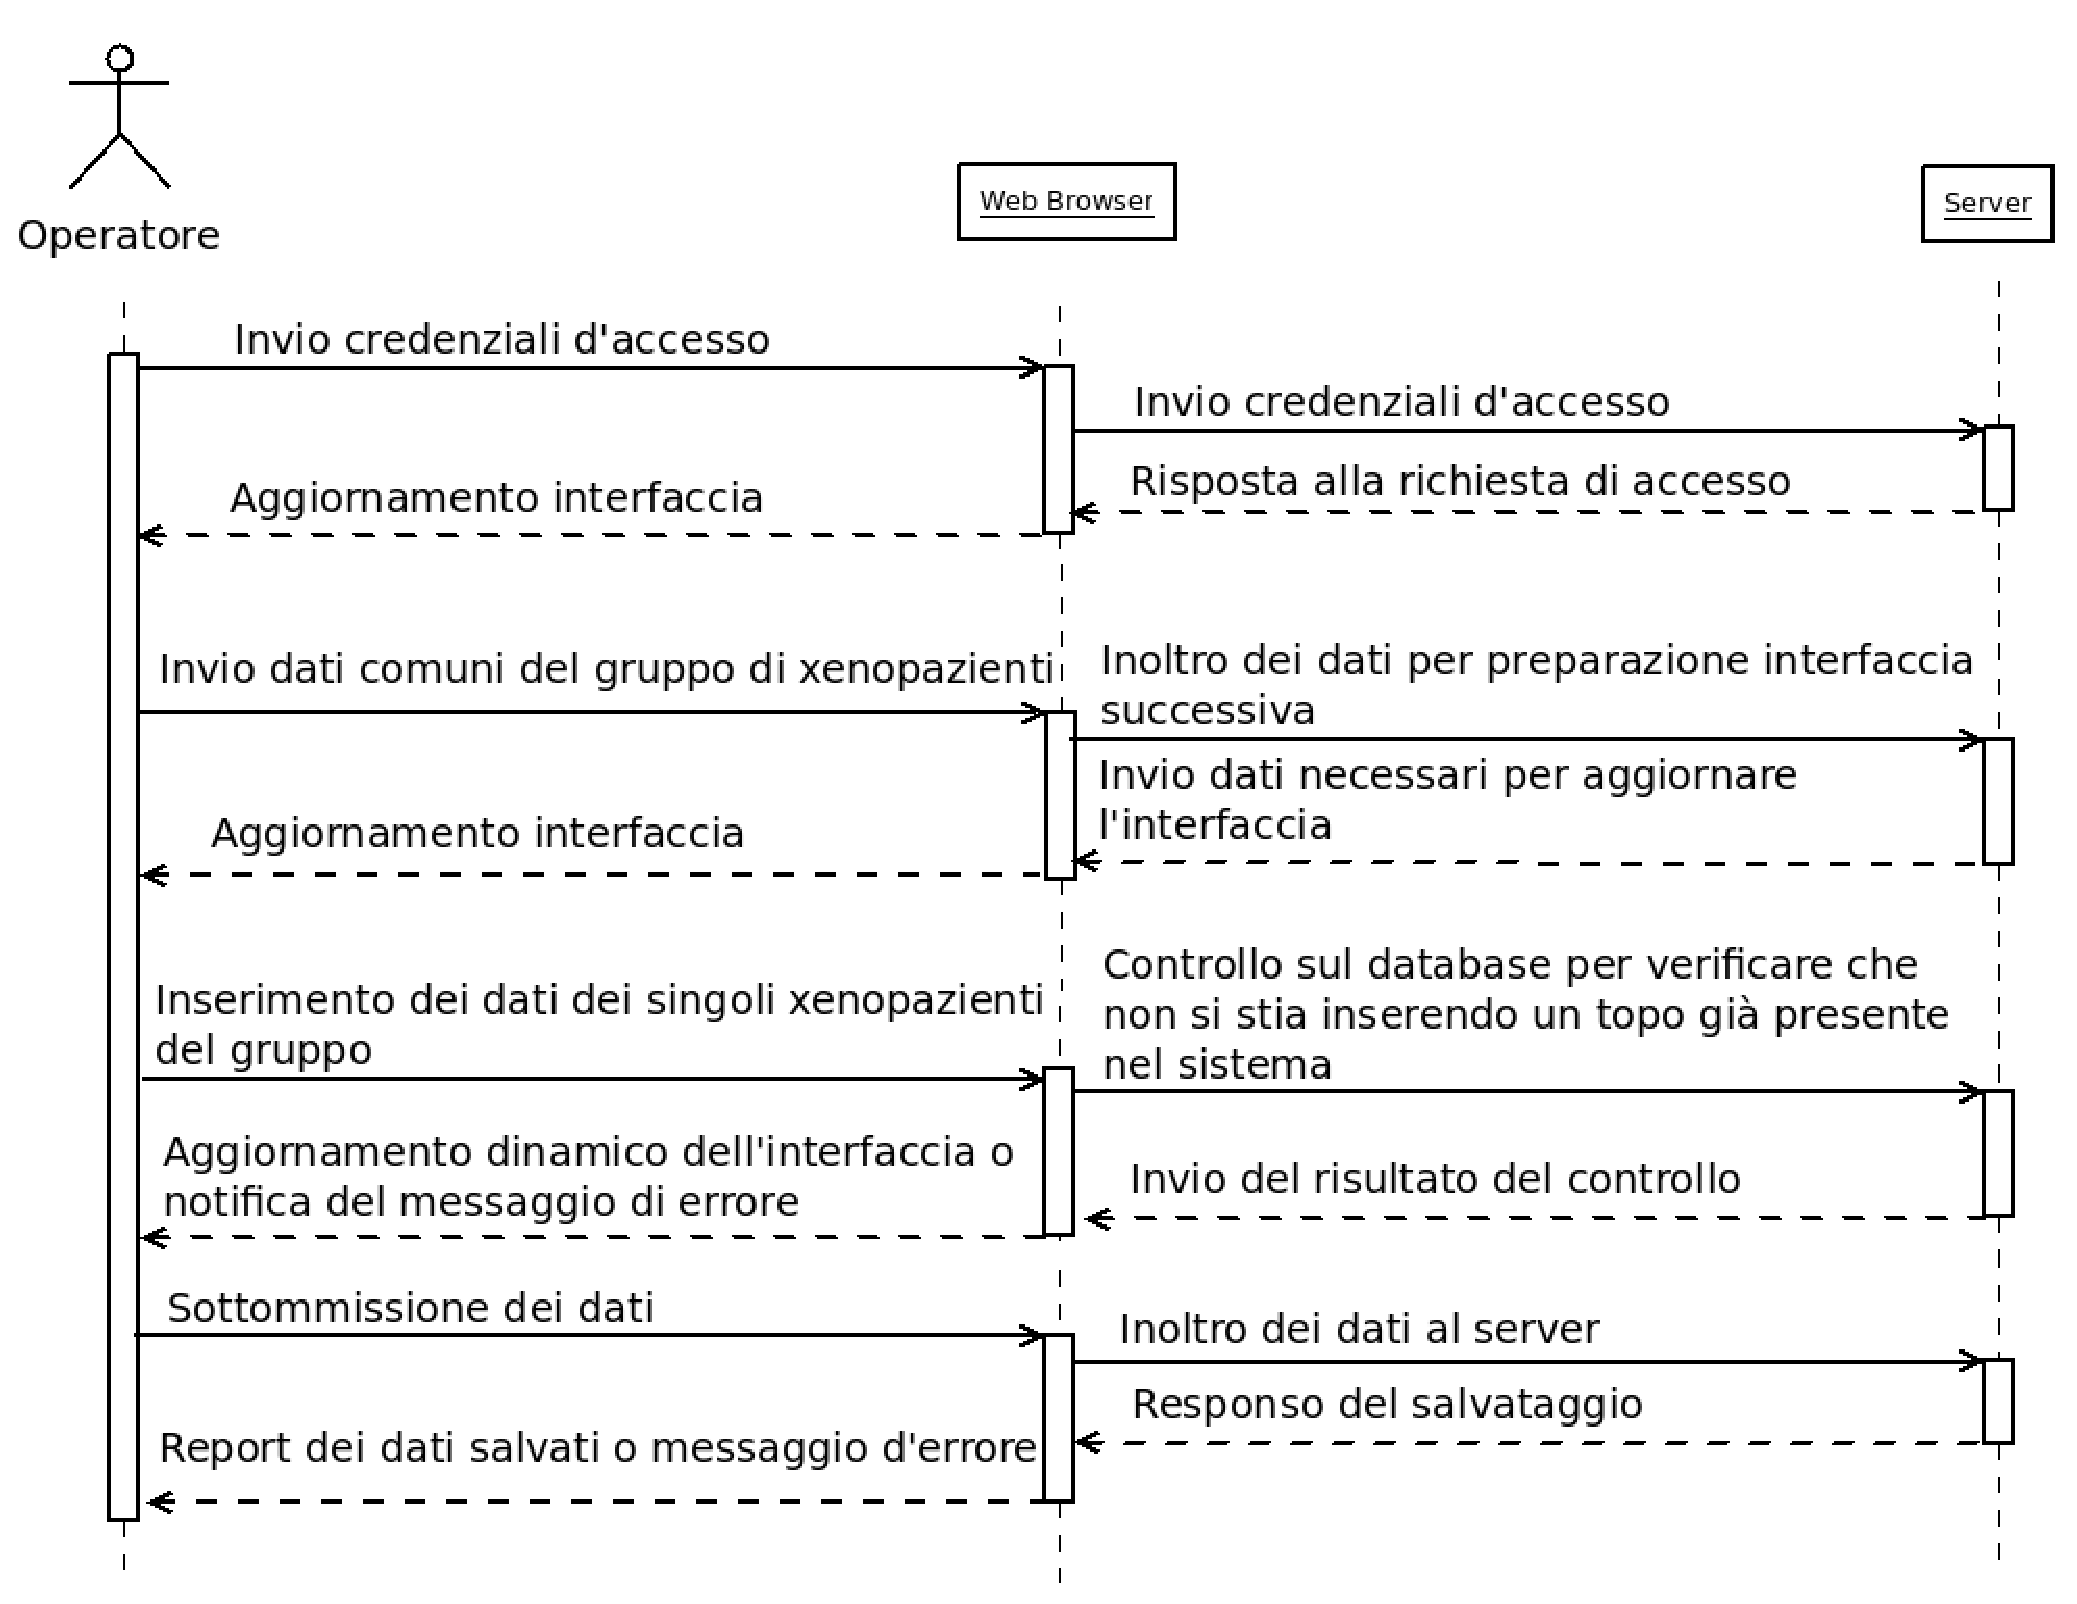
\includegraphics[width=0.7\textwidth]{./Figure/SDmiceloading}
\end{center}
\caption{Diagramma delle sequenze del caricamento xenopazienti\label{fig:SDmiceL}}
\end{figure}

\newpage

\section{Aggiornamento status degli xenopazienti}

Questa funzionalit\`a permette di cambiare lo status attuale ad uno o pi\`u xenopazienti, in modo tale da registrare il verificarsi di determinate situazioni, come ad esempio il trasferimento del topo o la morte non programmata. In Figura~\ref{fig:UCDmiceL} \`e riportato il diagramma dei casi d'uso relativo a questa interfaccia.

\begin{figure}[h]
\begin{center}
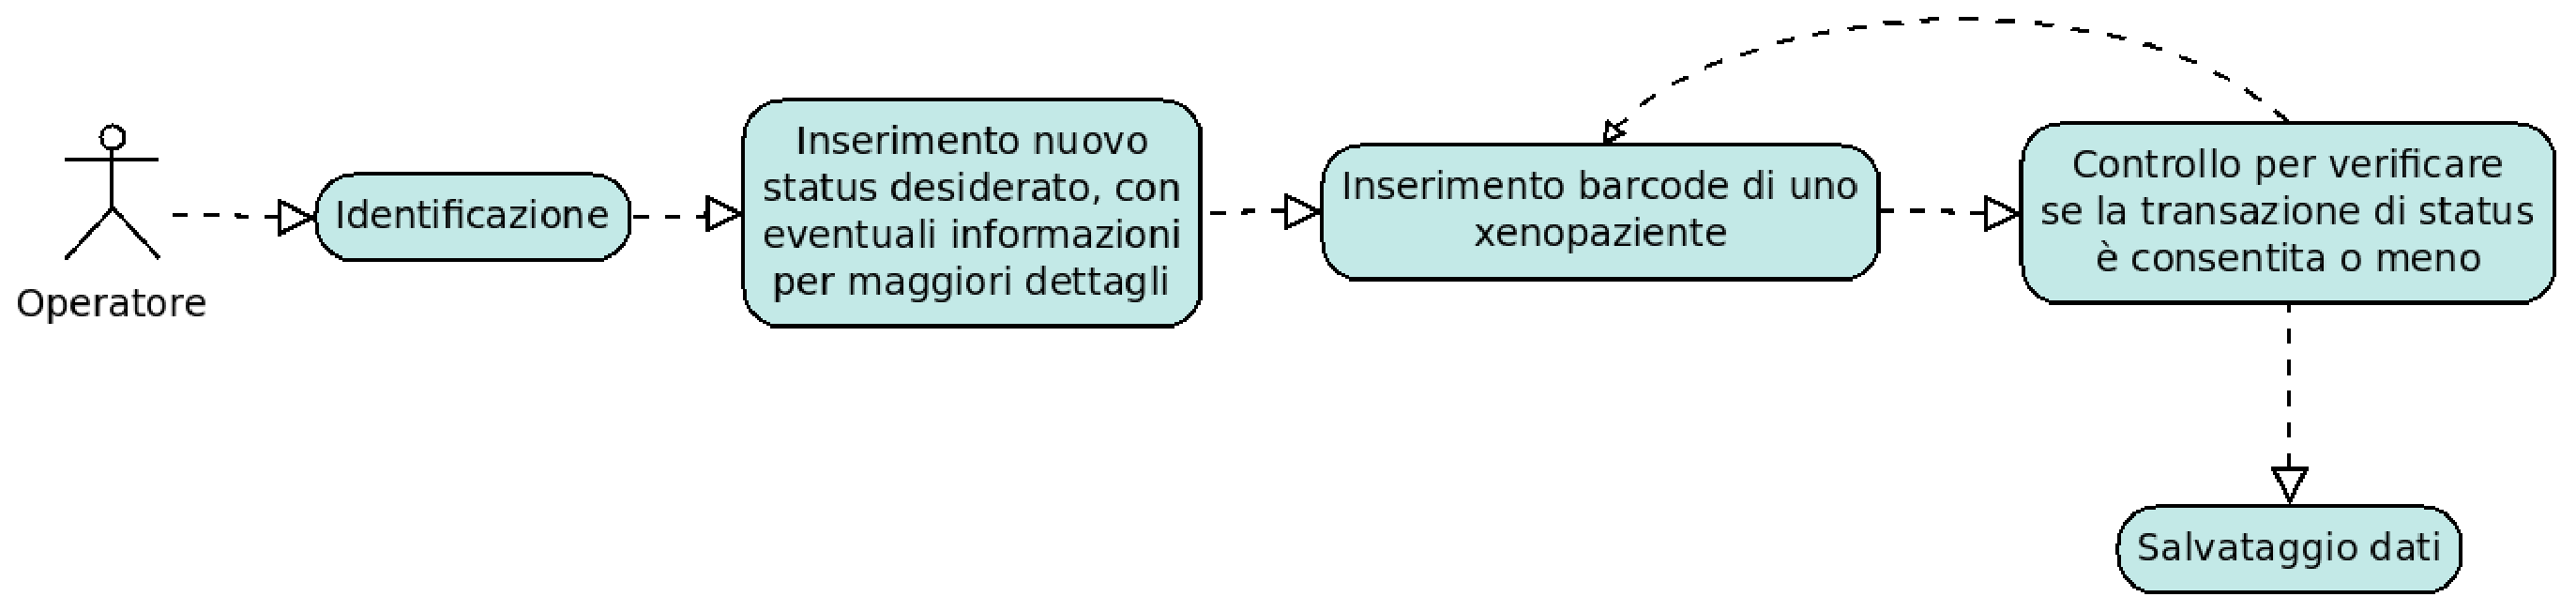
\includegraphics[width=0.8\textwidth]{./Figure/UCDchangestatus}
\end{center}
\caption{UCD dell'aggiornamento dello status degli xenopazienti\label{fig:UCDcs}}
\end{figure}

All'utente \`e inizialmente richiesto di immettere lo status da assegnare ad un gruppo di topi, inserito successivamente. Questa schermata gestisce i cambi si status non-ordinari, prelevando gli status proposti all'operatore dalla tabella Change\_status.
A seconda del nuovo status selezionato, verranno richieste o meno delle informazioni aggiuntive:
\begin{enumerate} 
	\item nel caso in cui il nuovo status sia \textit{dead accidentally}, si inseriscono la data di morte e delle eventuali note per i dettagli;
	\item nel caso in cui il nuovo status sia \textit{transferred}, si richiede il gruppo destinatario del topo.
\end{enumerate}

Successivamente, si presenta all'utente una semplice casella di testo, dove inserire il barcode di uno xenopaziente. L'inserimento pu\`o avvenire tramite tastiera o con l'apposito lettore di microchip, automatizzando l'immisione dei dati. Infatti, si associa il carattere return come suffisso ad ogni lettura di barcode. Quest'ultimo carattere consente di avviare, automaticamente e velocemente, la procedura per l'inserimento dei dati ricevuti. In questo modo, l'operatore pu\`o effettuare un aggiornamento di status di un grande gruppo di xenopazienti, in maniera veloce e automatica.

Per rimediare a eventuali errori di inserimento dati, si pu\`o utilizzare la lista degli aggiornamenti gi\`a impostati, come visto nella Sezione precedente.

L'amministratore del sistema, utilizzando l'interfaccia di amministrazione, pu\`o definire tutte le transizioni $<vecchio status \rightarrow nuovo status>$ non-ordinarie ammissibili per il sistema in uso, inserendole nella tabella Change\_status.

Nel momento in cui si finisce l'aggiornamento, si confermano i dati inseriti, visualizzando successivamente il report delle modifiche apportate al database o un messaggio di errore, a seconda dell'esito della transazione. In Figura~\ref{fig:SDcs} si pu\`o osservare il diagramma delle sequenze di questa interfaccia.

\begin{figure}[h]
\begin{center}
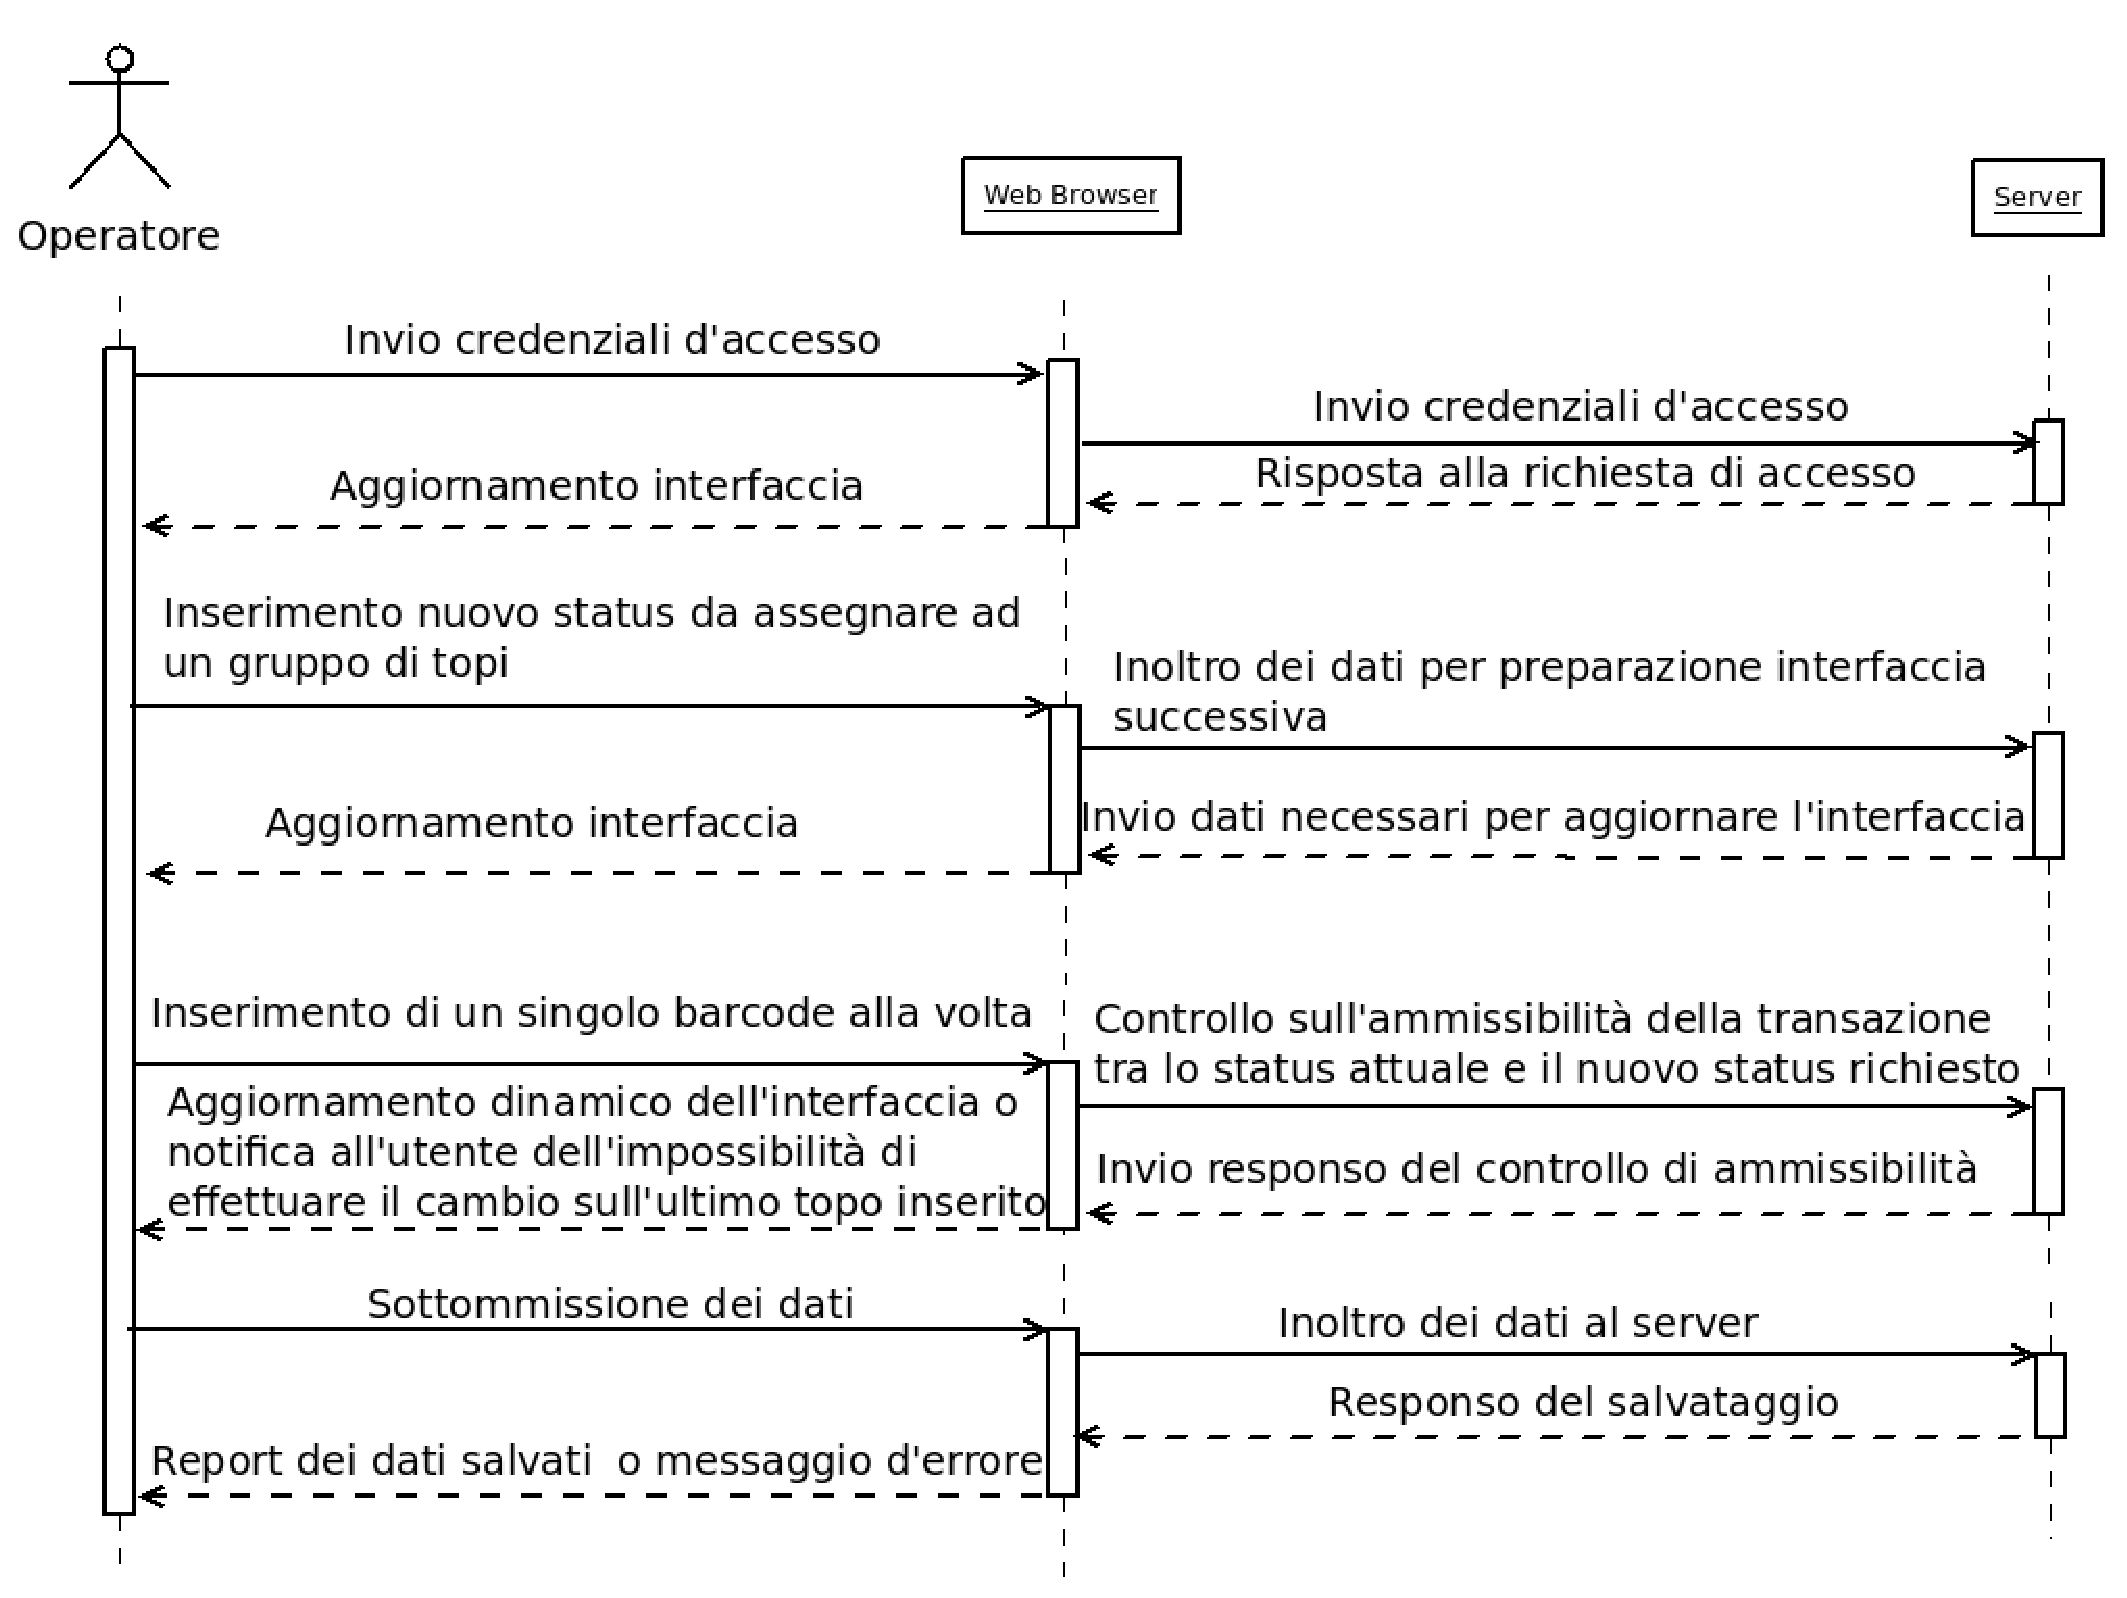
\includegraphics[width=0.6\textwidth]{./Figure/SDchangestatus}
\end{center}
\caption{Diagramma delle sequenze dell'aggiornamento dello status degli xenopazienti\label{fig:SDcs}}
\end{figure}

\newpage

\section{Misurazioni}

In questa Sezione si descrivono le interfacce per la gestione delle misure qualitative e quantitative. Queste due schermate sono molto simili tra di loro, quindi si \`e scelto di descriverle insieme, dettagliando successivamente le singole particolarit\`a. In Figura~\ref{fig:UCDmeasure} \`e riportato il relativo diagramma dei casi d'uso.

\begin{figure}[h]
\begin{center}
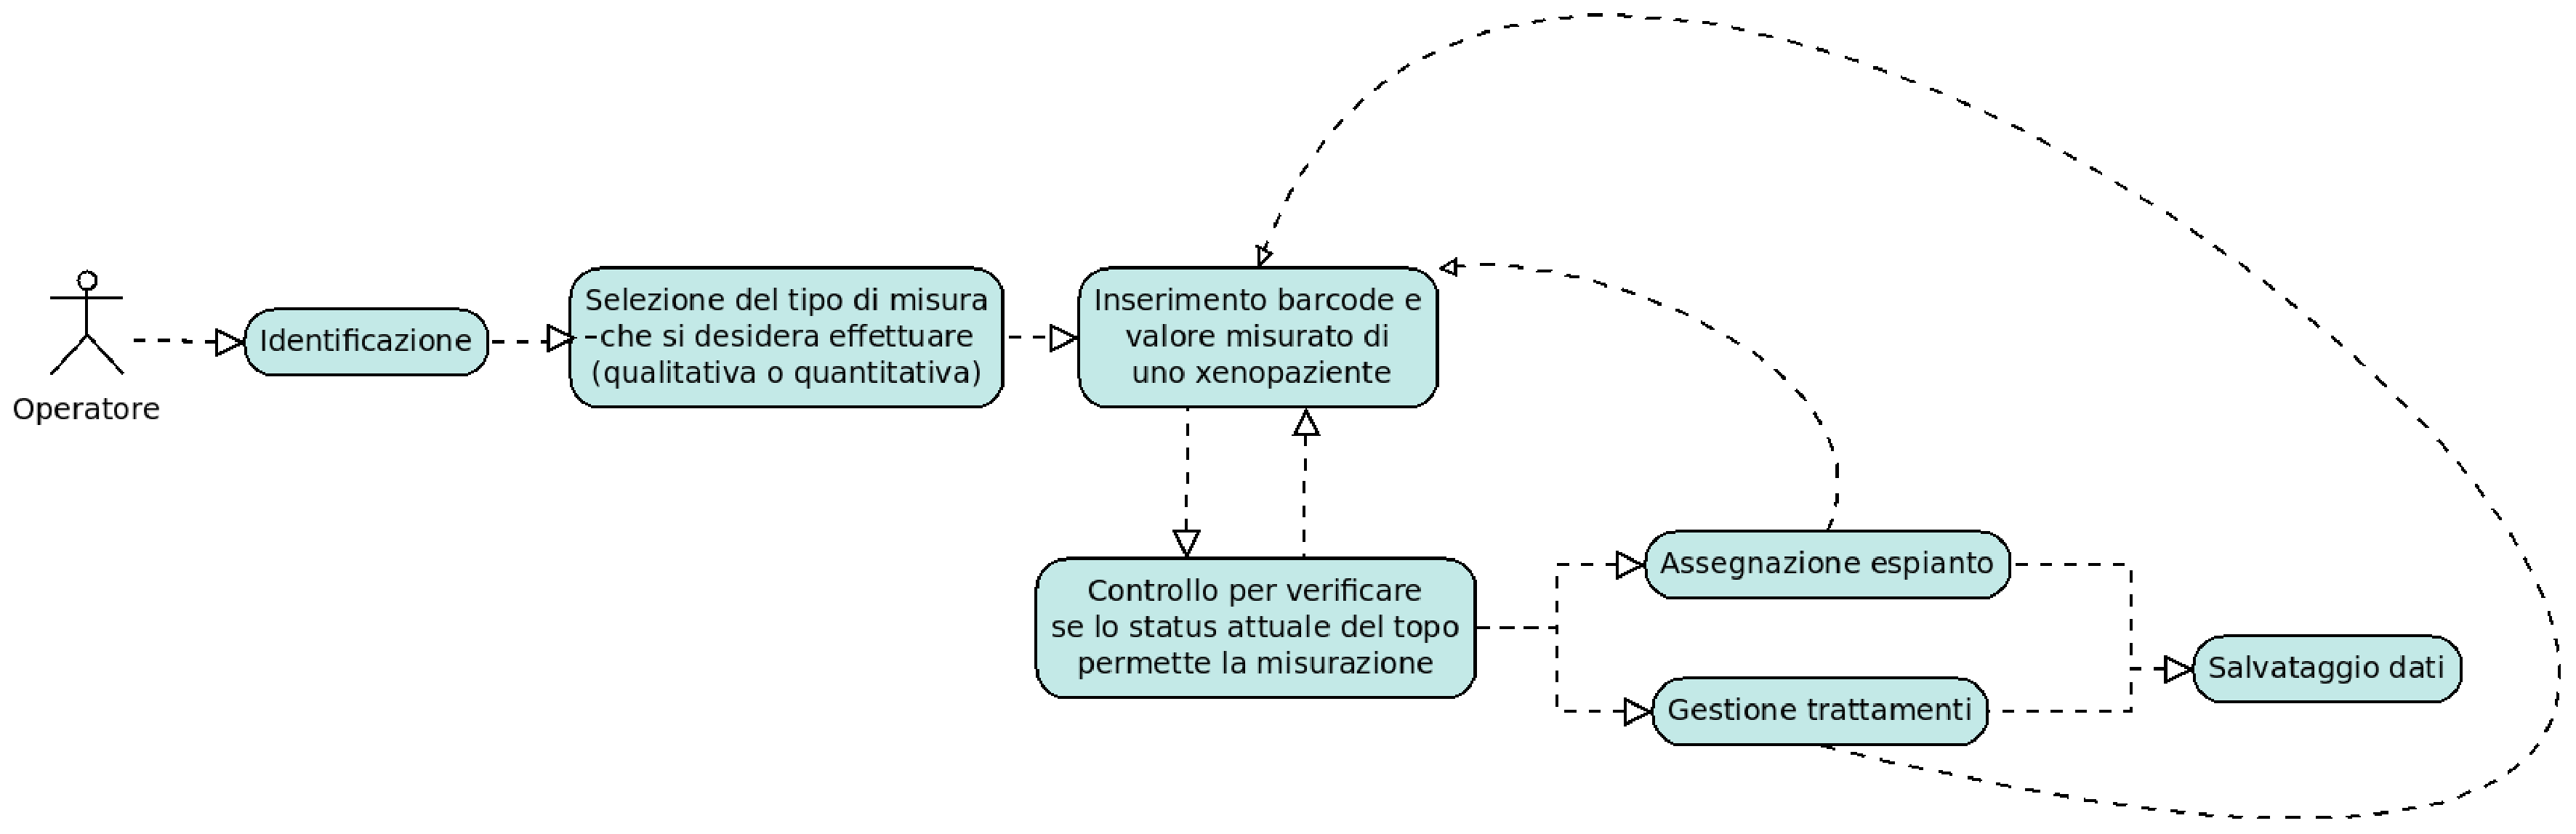
\includegraphics[width=0.9\textwidth]{./Figure/UCDmeasurements}
\end{center}
\caption{UCD delle operazioni di misurazioni\label{fig:UCDmeasure}}
\end{figure}

La somiglianza tra le due interfacce nasce sia perch\`e hanno poche differenze dal punto di vista della loro gestione, sia perch\`e si \`e cercato di mantenere il quanto pi\`u uguali possibili questi due template, per poter dare un ambiente pi\`u familiare all'utente che effettua sia misurazioni di un tipo, sia misurazioni dell'altro.

Nel momento in cui si accede alla schermata delle misurazioni, si specifica il tipo di misure che si vogliono collezionare. Attualmente, le misure consentite sono qualitative e quantitative. L'operatore, dopo aver scelto la tipologia delle misure che si intendono inserire nel database, raggiunge una schermata con una tabella, dove inserire i singoli dati delle varie misurazioni, tramite un apposito form di input. A causa dei vincoli operazionali, in questa tabella si possono inserire solo xenopazienti che hanno lo status \textit{implanted}.

Queste interfacce gestiscono il concetto delle meta-cage, visto nella Sezione~\ref{sec:contrMis}. Da questa tabella, si possono cancellare i topi inseriti, solo tra quelli dell'ultima meta-cage creata.

I campi di testo dove inserire i barcode degli xenopazienti da misurare, sono costruiti in modo tale che, dopo aver ricevuto il barcode dall'apposito lettore, venga automaticamente inserita una riga nell'apposita tabella. Quindi, il barcode \`e l'ultimo dato della misura da inserire, dopo aver immesso il valore relativo. Nel caso di misure quantitative, il valore della misura \`e ricevuto da un apposito calibro elettronico, il quale fornisce i due valori caratterizzanti questo tipo di misura. I campi di testo per questi due valori sono strutturati in modo tale da spostare il focus alla casella di testo successiva dopo aver ricevuto l'input dal calibro. Nella schermata delle misure quantitative, il valore da associare alla misurazione \`e prelevato da un elenco, contenente i dati presenti nella tabella \textit{Qualitative\_values}. Dopo aver inserito una misura di uno xenopaziente, si interroga il database attraverso delle API per verificare se il topo misurato ha un trattamento ad esso associato e se questo \`e acuto, oltre ai dati riguardanti la fine del trattamento stesso. Infine, si recuperano le informazioni su un eventuale espianto programmato sullo xenopaziente in questione.

L'obiettivo di queste due interfacce \`e, oltre a quello di collezionare i dati sulle varie misurazioni, fornire la possibilit\`a di programmare gli espianti sugli xenopazienti. L'espianto \`e programmato a discrezione dell'operatore, dopo che ha valutato la misura effettuata. Inoltre, si svolge anche il compito della gestione dei trattamenti; infatti, da qui si possono gestire i trattamenti sui topi, dopo averli selezionati e cliccando sui tasti per iniziare o fermare un trattamento. L'interfaccia dei trattamenti \`e illustrata nella sezione seguente.

Per le misure quantitave, \`e presente un campo di testo che visualizza la media di tutte le misure inserite nella meta-cage corrente. Inoltre, \`e anche possibile visualizzare la media delle sole righe selezionate, per poter verificare i valori medi di precisi gruppi di xenopazienti. Chiaramente, questo concetto di media non \`e applicabile alle misure qualitative, in quanto si raccolgono valori categorici. Per gestire la media, \`e presente anche un valore di soglia, il quale rappresenta un limite massimo. Nel momento in cui il valore di una media supera questa soglia, le caselle di testo contenenti le due medie si colorano di rosso, in modo tale da fornire un valore pi\`u visibile all'operatore. Per elasticizzare maggiormente il sistema, il valore di soglia \`e modificabile dinamicamente dall'operatore. In Figura~\ref{fig:qm} si pu\`o osservare quanto appena descritto.

\begin{figure}[h]
\begin{center}
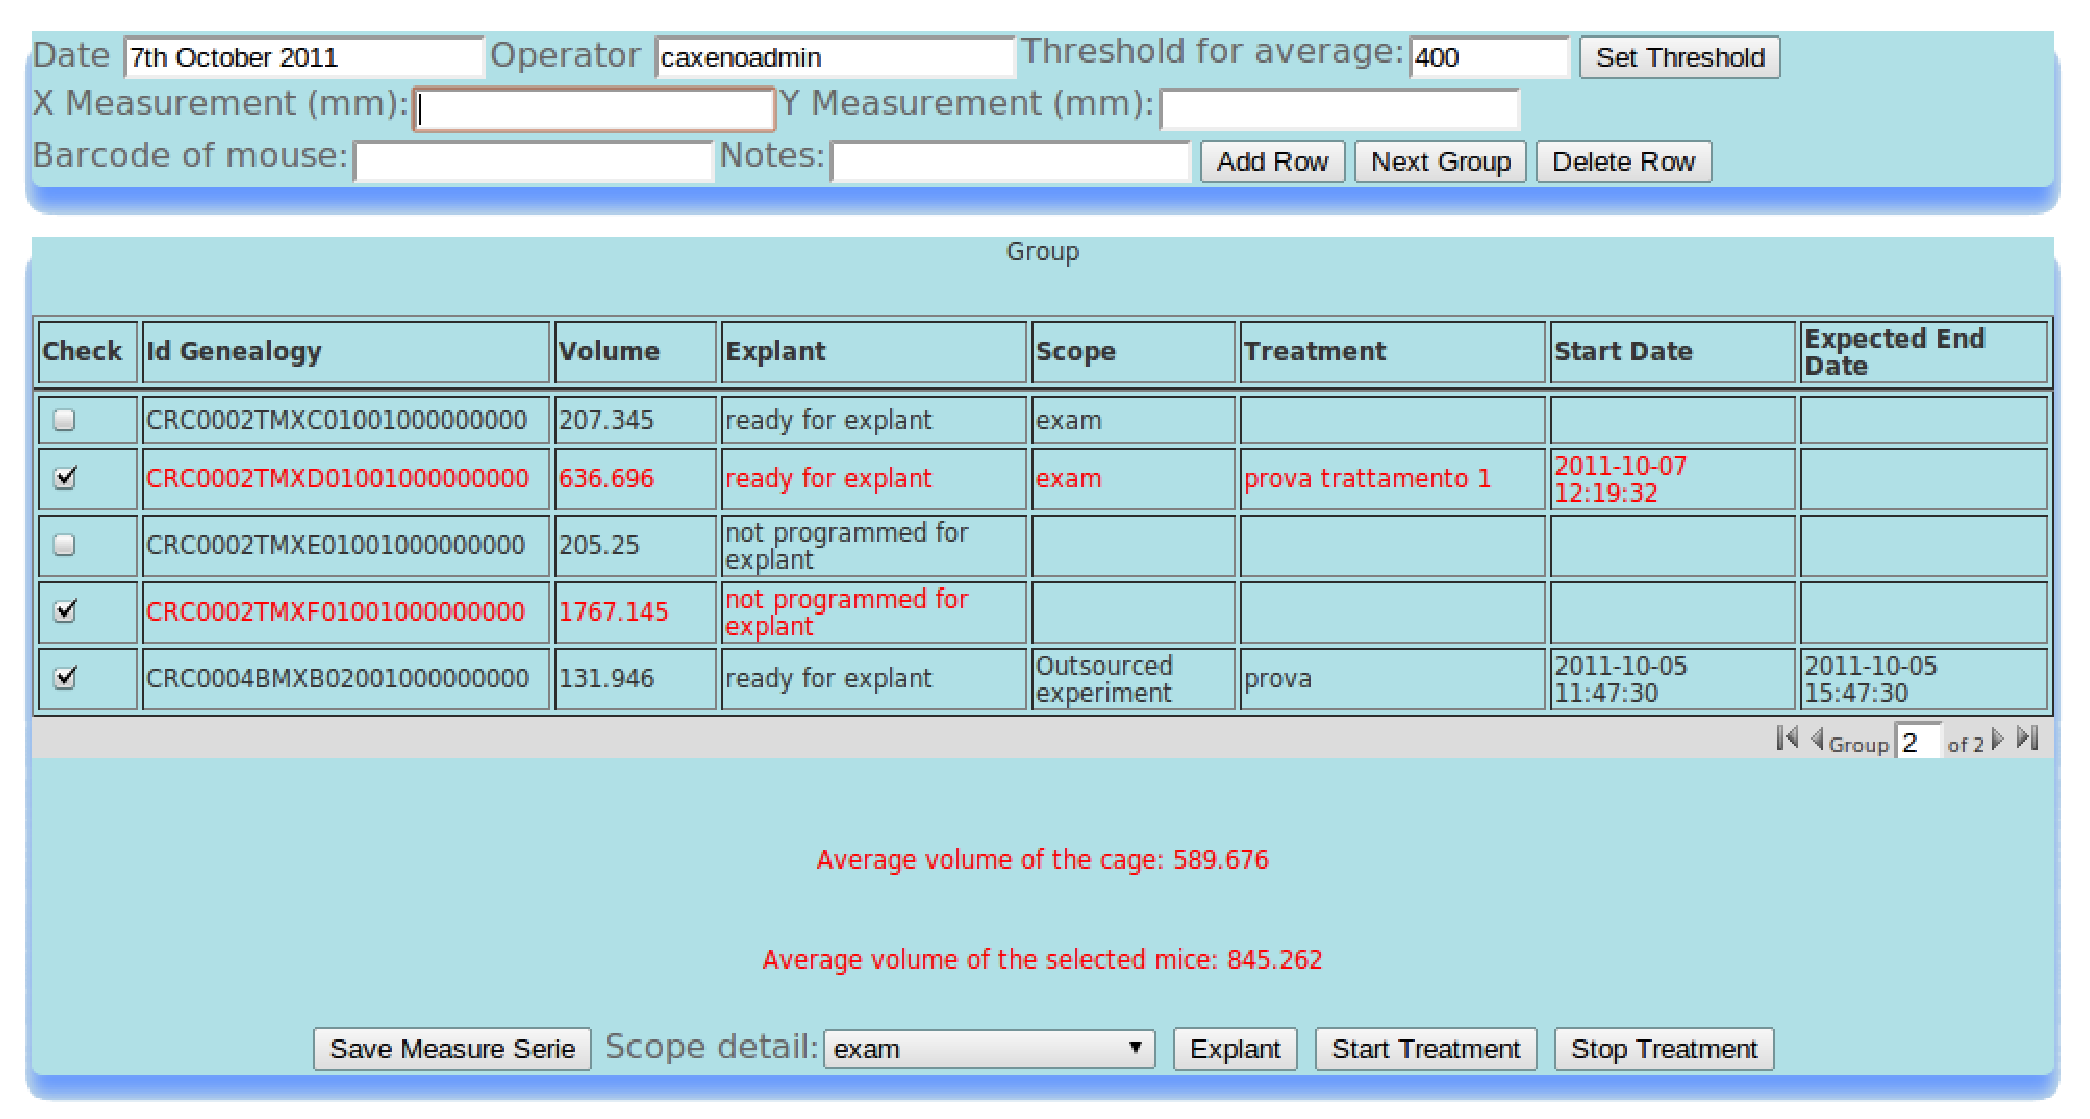
\includegraphics[width=1.0\textwidth]{./Figure/quantMeasure}
\end{center}
\caption{Schermata per la collezione di misure quantitative\label{fig:qm}}
\end{figure}

In Figura~\ref{fig:SDmeasure} si pu\`o osservare il diagramma delle sequenze per la collezione dei dati delle misurazioni.

\begin{figure}[h]
\begin{center}
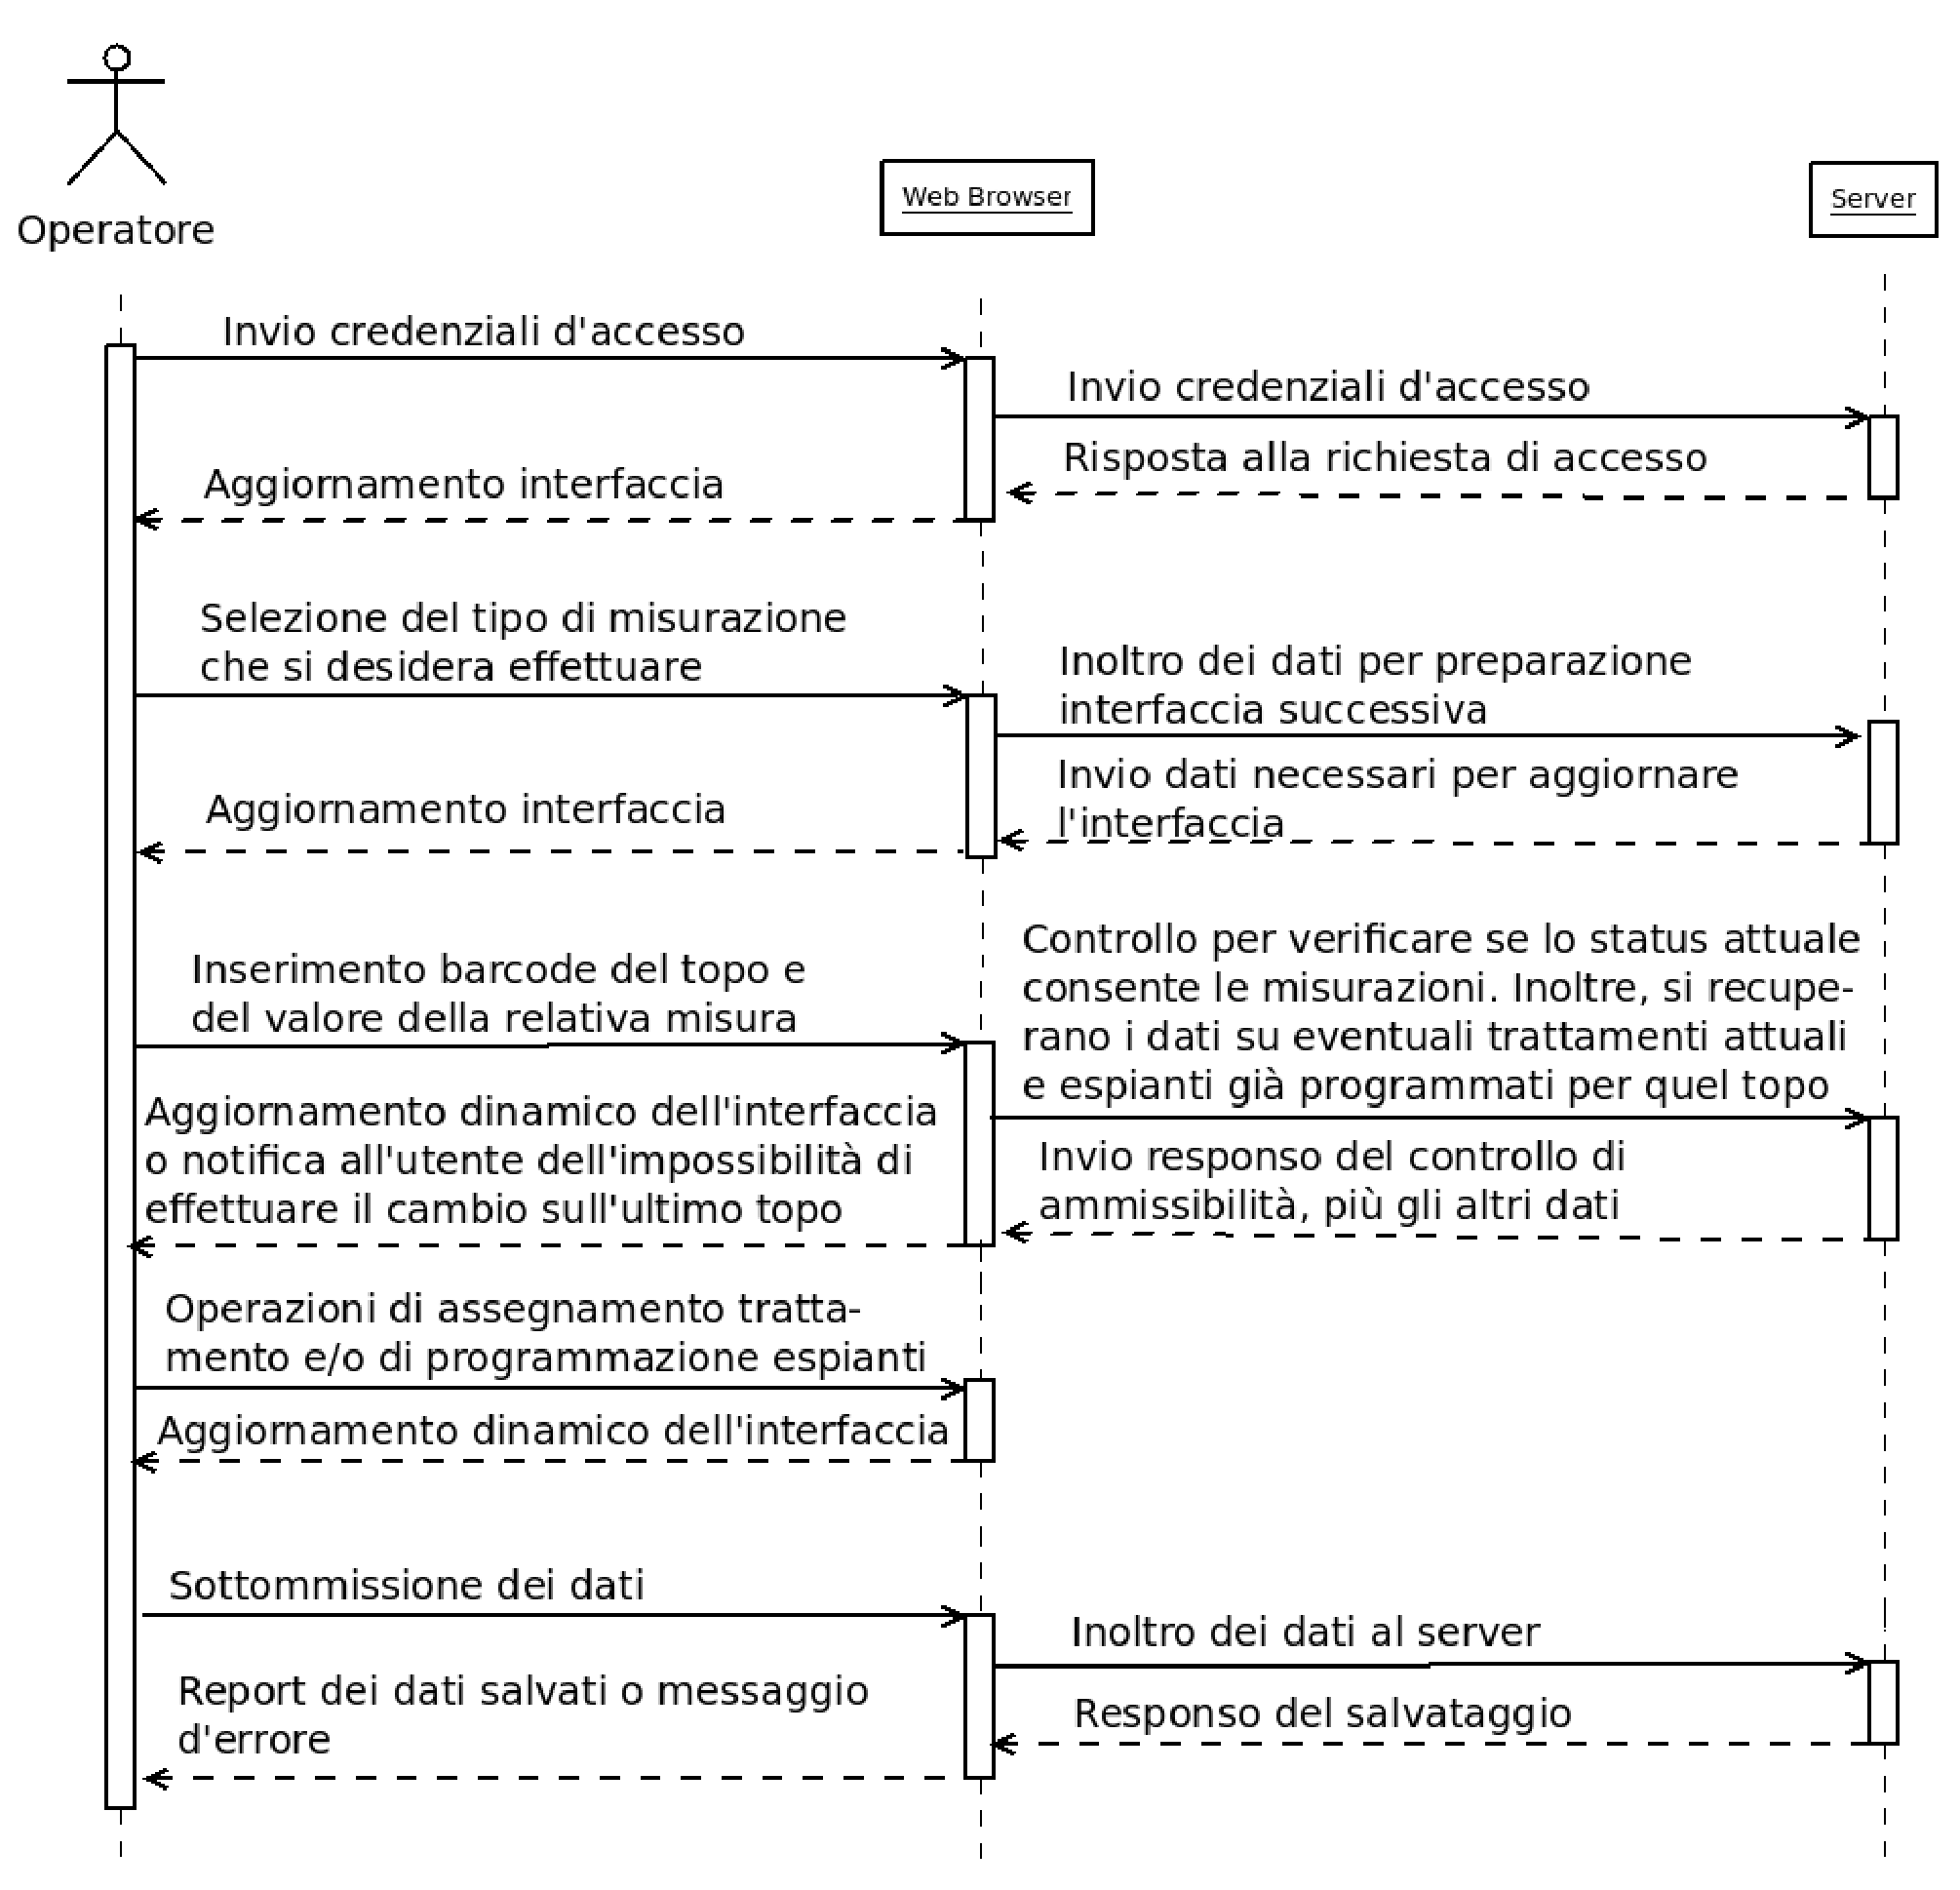
\includegraphics[width=0.6\textwidth]{./Figure/SDmeasurements}
\end{center}
\caption{Diagramma delle sequenze della gestione delle operazioni delle misurazioni\label{fig:SDmeasure}}
\end{figure}

\newpage

\section{Gestione trattamenti}\label{sec:tratt}

Questa interfaccia \`e accessibile solo dopo aver effettuato delle misure su uno o pi\`u xenopazienti. Infatti, dopo averli misurati, se ne seleziona almeno uno dalla tabella, per poi entrare nella finestra per gestire i trattamenti. Sfruttando questo legame con le misurazioni, il diagramma dei casi d'uso dei trattamenti (Figura~\ref{fig:UCDtreat}) pu\`o essere visto come l'espansione del nodo `Gestione trattementi' dell'UCD in Figura~\ref{fig:UCDmeasure}.

\begin{figure}[h]
\begin{center}
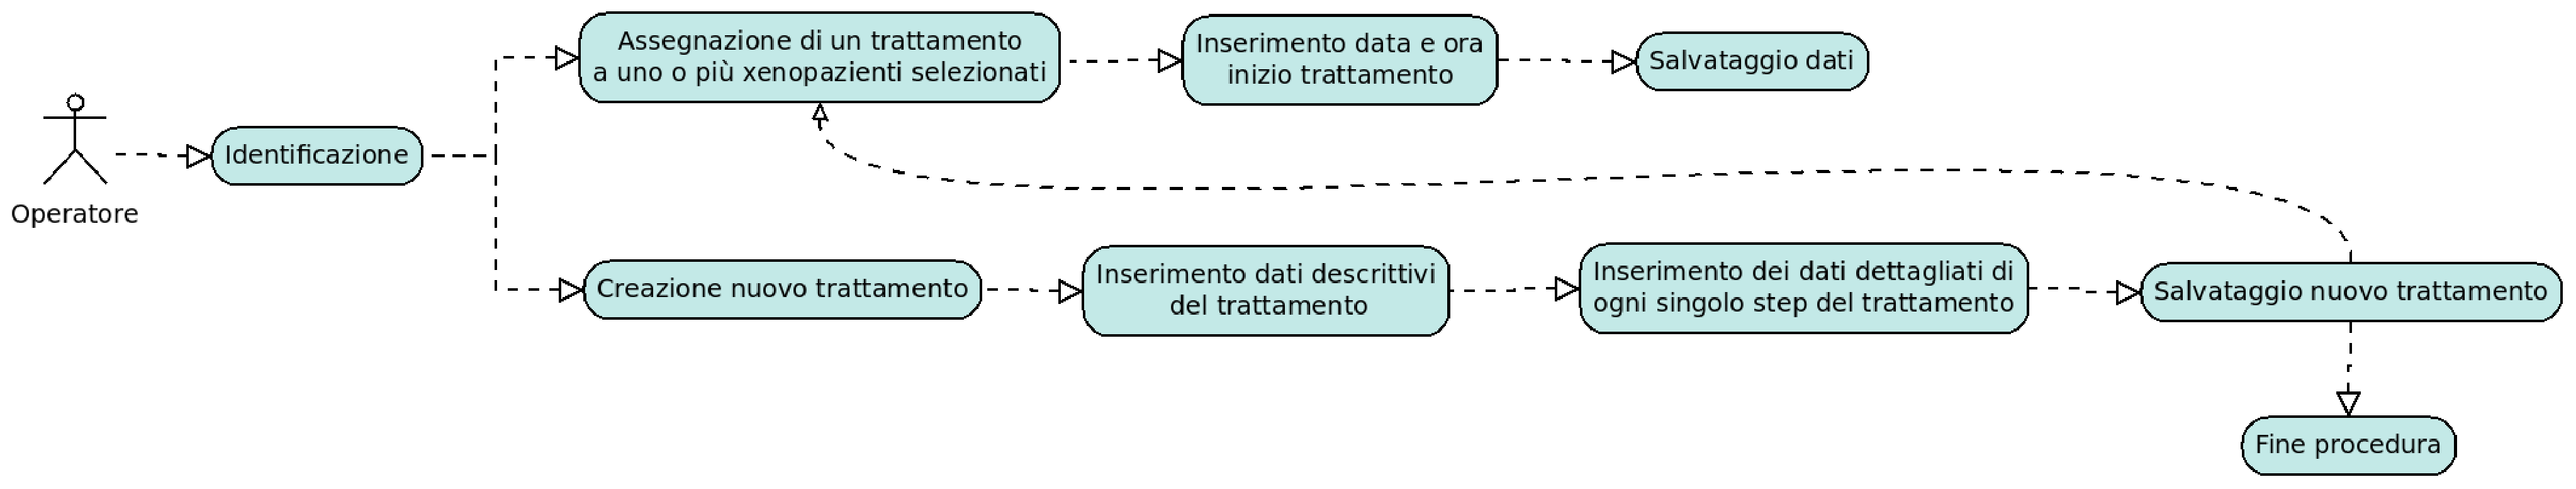
\includegraphics[width=0.9\textwidth]{./Figure/UCDtreatments}
\end{center}
\caption{UCD della gestione dei trattamenti\label{fig:UCDtreat}}
\end{figure}

Nel momento in cui si effettua una misura su uno xenopaziente impiantato, si presenta la possiblit\`a di gestirne i trattamenti. Partendo da ci\`o che offre l'interfaccia, le possibilit\`a sono:
\begin{itemize}
	\item \textbf{avvio trattamento}: si decide di avviare un trattamento su un topo che non ha gi\`a un trattamento in corso. Per sottoporre un topo ad un trattamento, l'utente pu\`o selezionare un trattamento tra quelli esistenti oppure crearne uno ad hoc, rendendolo cos\`i disponibile per eventuali usi futuri. \`E possibile quindi applicare pi\`u volte lo stesso trattamento a diversi topi, in modo tale da poter confrontare i risultati sperimentali ottenuti su soggetti diversi;
	\item \textbf{interruzione trattamento}: se si reputa inutile il proseguimento di un trattamento, lo si pu\`o interrompere prima della sua scadenza programmata. Questa operazione \`e svolta senza accedere direttamente all'interfaccia creata per la gestione delle misurazioni;
	\item \textbf{stop\&start trattamento}: questa possibilit\`a \`e la combinazione delle due precedenti, utilizzata nel caso in cui si voglia applicare un trattamento diverso da quello attuale.
\end{itemize}

Per avviare un nuovo trattamento, si accede all'apposita interfaccia. Per scegliere il trattamento da cominciare, si accede ad un elenco di trattamenti disponibili. Inoltre si ha la possibilit\`a di scegliere quando farlo cominciare. Se in questa lista non \`e presente ci\`o che si desidera, si avvia la procedura per crearne uno nuovo, per poi assegnarlo agli xenopazienti precedentemente selezionati.

Nel momento in cui si crea un nuovo trattamento, se ne inseriscono i dati descrittivi, quali il nome, una breve descrizione, la durata e la tipologia di trattamento a cui appartiente. Il nome assegnato al nuovo trattamento deve essere univoco. Per assicurare questo vincolo, si \`e implementato un'apposita API per verificare i dati gi\`a presenti nel database. Le tipologie dei trattamenti sono, attualmente, due: i trattementi base e i trattamenti acuti. Questi ultimi hanno la particolarit\`a che, una volta interrotti o terminati, implicano un espianto forzato degli xenopazienti sui quali \`e stato applicato.

Specificare la durata e la sua unit\`a di misura, serve per creare, successivamente, il diagramma di Gantt (strumento di supporto alla gestione dei progetti\cite{gantt}) per programmare nel dettaglio i vari passaggi del trattamento che si sta creando. L'utente pu\`o dinamicamente aggiungere varie righe, dove ognuna di questa rappresenta un determinato passaggio del trattamento, caratterizzato dal farmaco e dal modo in cui viene somministrato, dalla dose e dal numero di volte che deve essere utilizzato nell'unit\`a di tempo precedentemente selezionata (ad esempio, 2 volte ogni ora o 1 al giorno), dove ogni colonna costituisce uno slot temporale, come illustrato in Figura~\ref{fig:gantt}. Dopo aver inserito le righe desiderate, ci si ritrova con una tabella dove ogni cella corrisponde a una determinata somministrazione in un certo slot temporale. Selezionando le celle, si pu\`o cos\`i creare un trattamento composto da molteplici step molto dettagliati. Se si sbaglia ad inserire una riga, \`e sufficiente lasciarla vuota per fare in modo che non venga salvata nel database. Una volta salvato il trattamento, e dopo aver ricevuto un messaggio di conferma, si torna alla schermata precedente, dove si pu\`o ora selezionare il nuovo trattamento ed assegnarlo agli xenopazienti. In Figura~\ref{fig:SDtreat} si pu\`o osservare il diagramma delle sequenze di questa interfaccia.

\begin{figure}[h]
\begin{center}
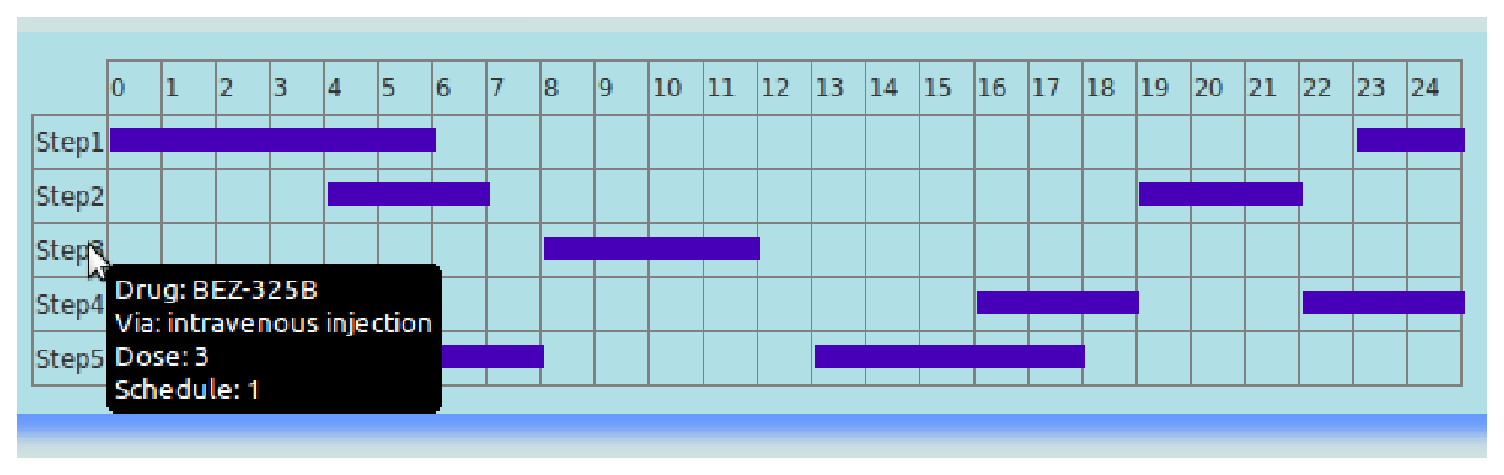
\includegraphics[width=1.0\textwidth]{./Figure/gantt}
\end{center}
\caption{Esempio di utilizzo del diagramma di Gantt in XMS\label{fig:gantt}}
\end{figure}

\begin{figure}[h]
\begin{center}
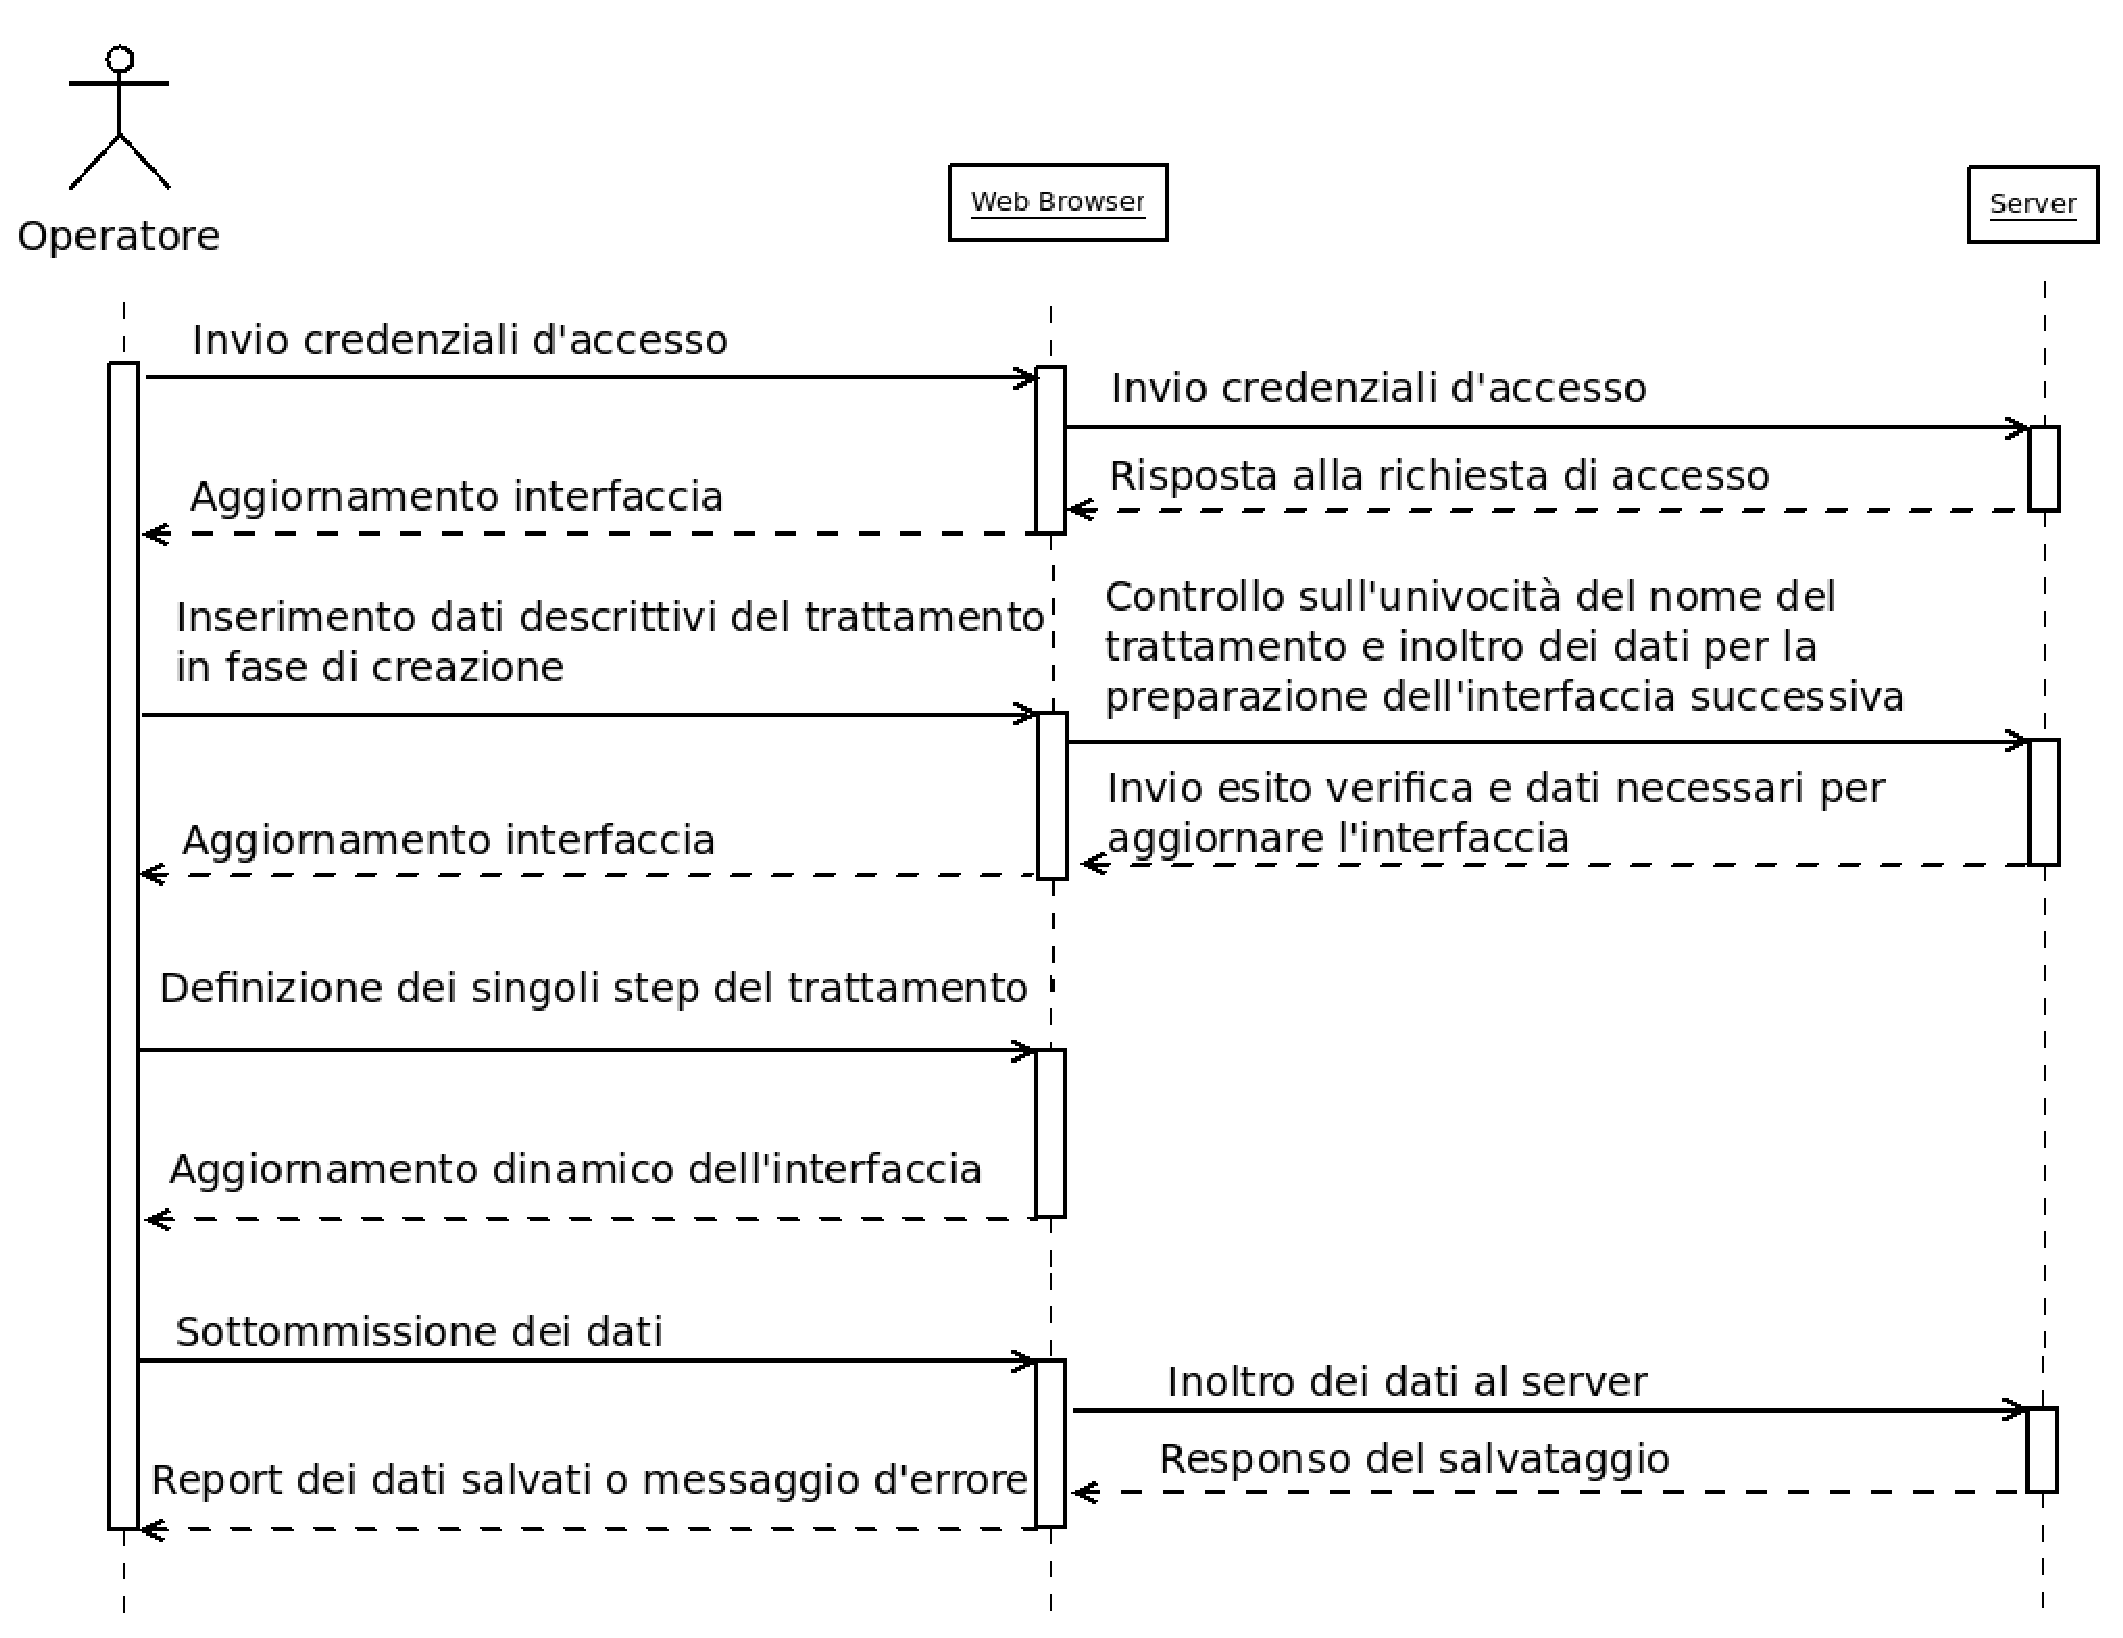
\includegraphics[width=0.6\textwidth]{./Figure/SDtreatmentsCreate}
\end{center}
\caption{Diagramma delle sequenze delle operazioni effettuate per creare un trattamento\label{fig:SDtreat}}
\end{figure}

\newpage

\section{Impianti}

Considerando l'ordine temporale delle operazioni svolte su uno xenopaziente nel suo ciclo di vita, la gestione degli impianti \`e la prima dove si \`e cercato di simulare l'ambiente di laboratorio. In Figura~\ref{fig:UCDimpl} \`e riportato il diagramma dei casi d'uso relativo a questa interfaccia.

\begin{figure}[h]
\begin{center}
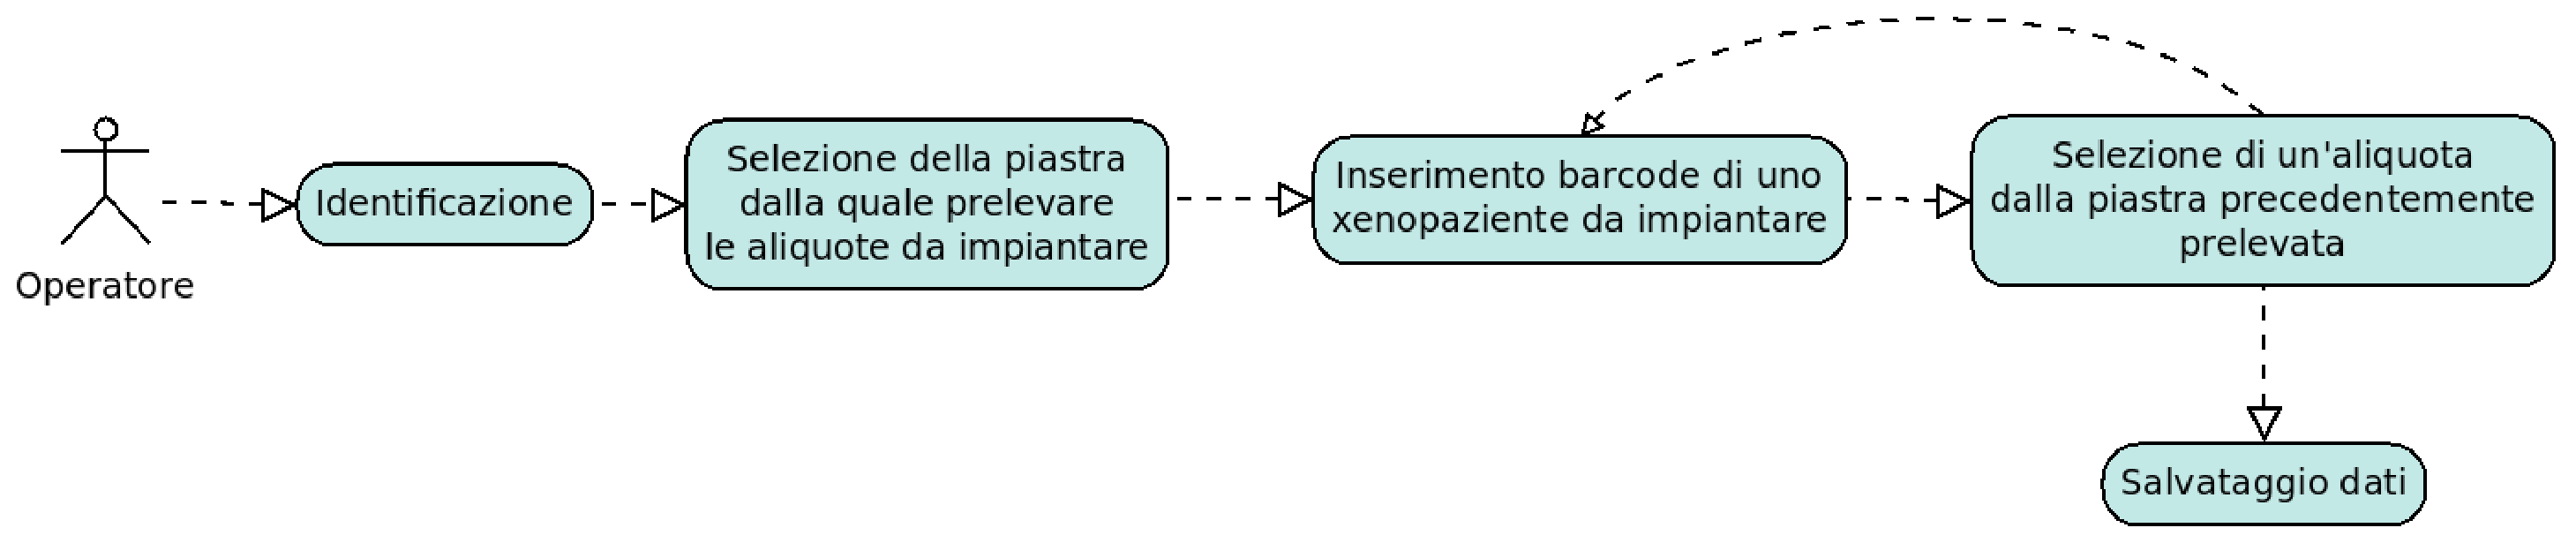
\includegraphics[width=0.8\textwidth]{./Figure/UCDimplants}
\end{center}
\caption{UCD relativo agli impianti\label{fig:UCDimpl}}
\end{figure}

Nel database, le informazioni relative ad un determinato insieme di impianti sono tra loro collegate tramite una serie, conetto utilizzato per raggruppare gli impianti svolti nella stessa sessione operativa (stessa piastra sorgente, data e operatore). Anche l'utente \`e cosciente di questo concetto, grazie alla struttura con la quale \`e stata costruita l'interfaccia degli impianti. Infatti, prima di inserire i dettagli di ogni singola operazione, vengono richiesti i dati comuni a tutta la serie di operazioni: la data dell'impianto e un eventuale commento. Inoltre, molto importante, si inserisce il barcode della piastra dalla quale si intendono prelevare le aliquote da impiantare. Questo barcode viene inoltrato alla BioBanaca, la quale, tramite apposite API, invia al \Xeno\ le informazioni riguardanti la piastra richiesta e le aliquote eventualmente contenute in essa. Grazie a questo scambio di informazioni, si \`e in grado di costruire un tabella che simula la piastra e la disposizione delle provette all'interno di essa, dalla quale l'utente pu\`o selezionare l'aliquota da impiantare nel topo. Dopo aver inserito i dati preliminari, si accede alla schermata nella quale definire i singoli impianti. In questa interfaccia possono essere utilizzati solo xenopazienti aventi lo status \textit{experimental}. Se si cerca di utilizzare un topo che non appartiente a questo status, si notifica un messaggio all'operatore.

Per la simulazione della piastra, \`e stata creata una tabella rappresentante una piastra, dove ogni cella simula una provetta, contenente una determinata aliquota. Si \`e inserito un numero per ogni cella, rappresentante la quantit\`a di frammenti della stessa aliquota presente in quella provetta. Inoltre, \`e stato implementato un sistema cromatico, con un colore associato ad ogni cella, per poter visionare velocemente la situazione della piastra. In Figura~\ref{fig:implantP} se ne pu\`o vedere un esempio, mentre di seguito si elencano e descrivono i colori utilizzati:
\begin{enumerate} 
  \item giallo chiaro: \`e presente almeno un'aliquota nella provetta rappresentata da questa cella;
  \item nero: non \`e presenta alcuna aliquota;
  \item giallo scuro: sono finite le aliquote inizialmente presenti in quella cella;
  \item azzurro: l'aliquota \`e attualmente selezionata.
\end{enumerate} 

\noindent Appena \`e selezionata un'aliquota, nella pagina viene visualizzato il suo identificativo di genealogia e il nuovo identificativo di genealogia da essa creato, che sar\`a assegnato allo xenopaziente impiantato con quel tessuto.

\begin{figure}[h]
\begin{center}
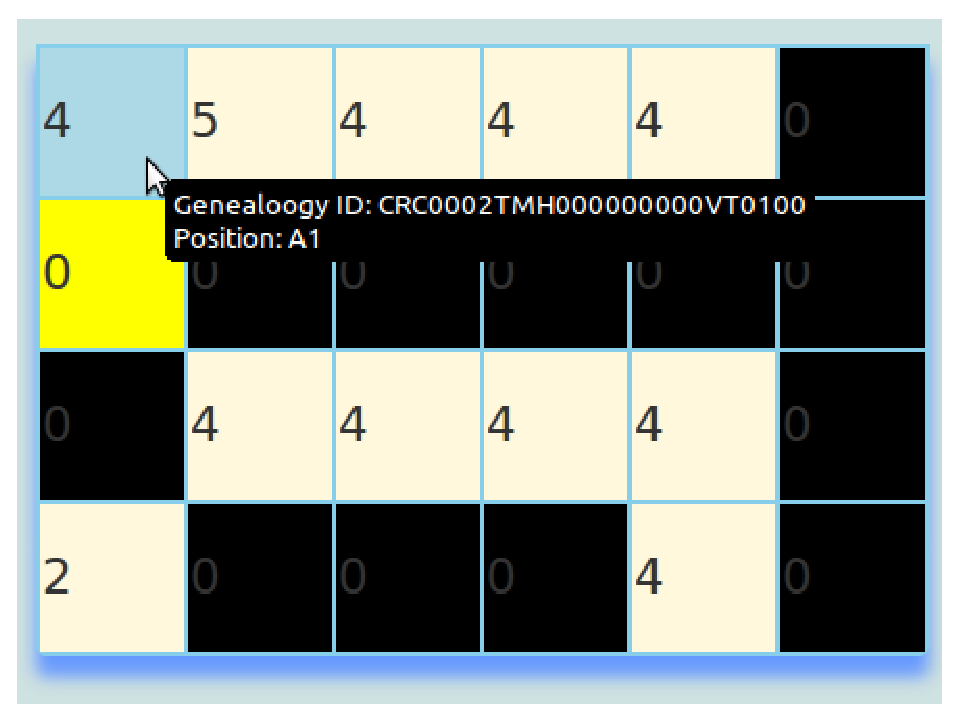
\includegraphics[width=0.6\textwidth]{./Figure/implantPlate}
\end{center}
\caption{Utilizzo della tabella contenente i dati delle aliquote\label{fig:implantP}}
\end{figure}

Oltre a selezionare l'aliquota, si deve anche selezionare il topo, il sito dell'impianto e settare eventualmente il BadQualityFlag (il quale indica un impianto mal riuscito). Una volta selezionati sia l'aliquota, sia lo xenopaziente (non necessariamente in questo ordine), si pu\`o procedere ad inserire l'impianto appena impostato nella tabella riepilogativa, dalla quale, in caso di errore, si possono cancellare le righe relative alle operazioni errate. Quando l'inserimento dati \`e terminato, si pu\`o completare la serie di impianti cliccando su `Save'. Se la piastra impiegata ha ancora aliquote al suo interno, si chiede all'utente se si desidera svuotarne il contenuto. Dopodich\`e, in caso di esito positivo della transazione, si visualizza il report dei dati appenna immessi nel database. Inoltre, si invia la lista delle aliquote utilizzate alla \Tissue\ e l'informazione relativa all'eventuale svuotamento della piastra. In Figura~\ref{fig:SDimpl} si pu\`o osservare il diagramma delle sequenze di questa interfaccia.

\begin{figure}[h]
\begin{center}
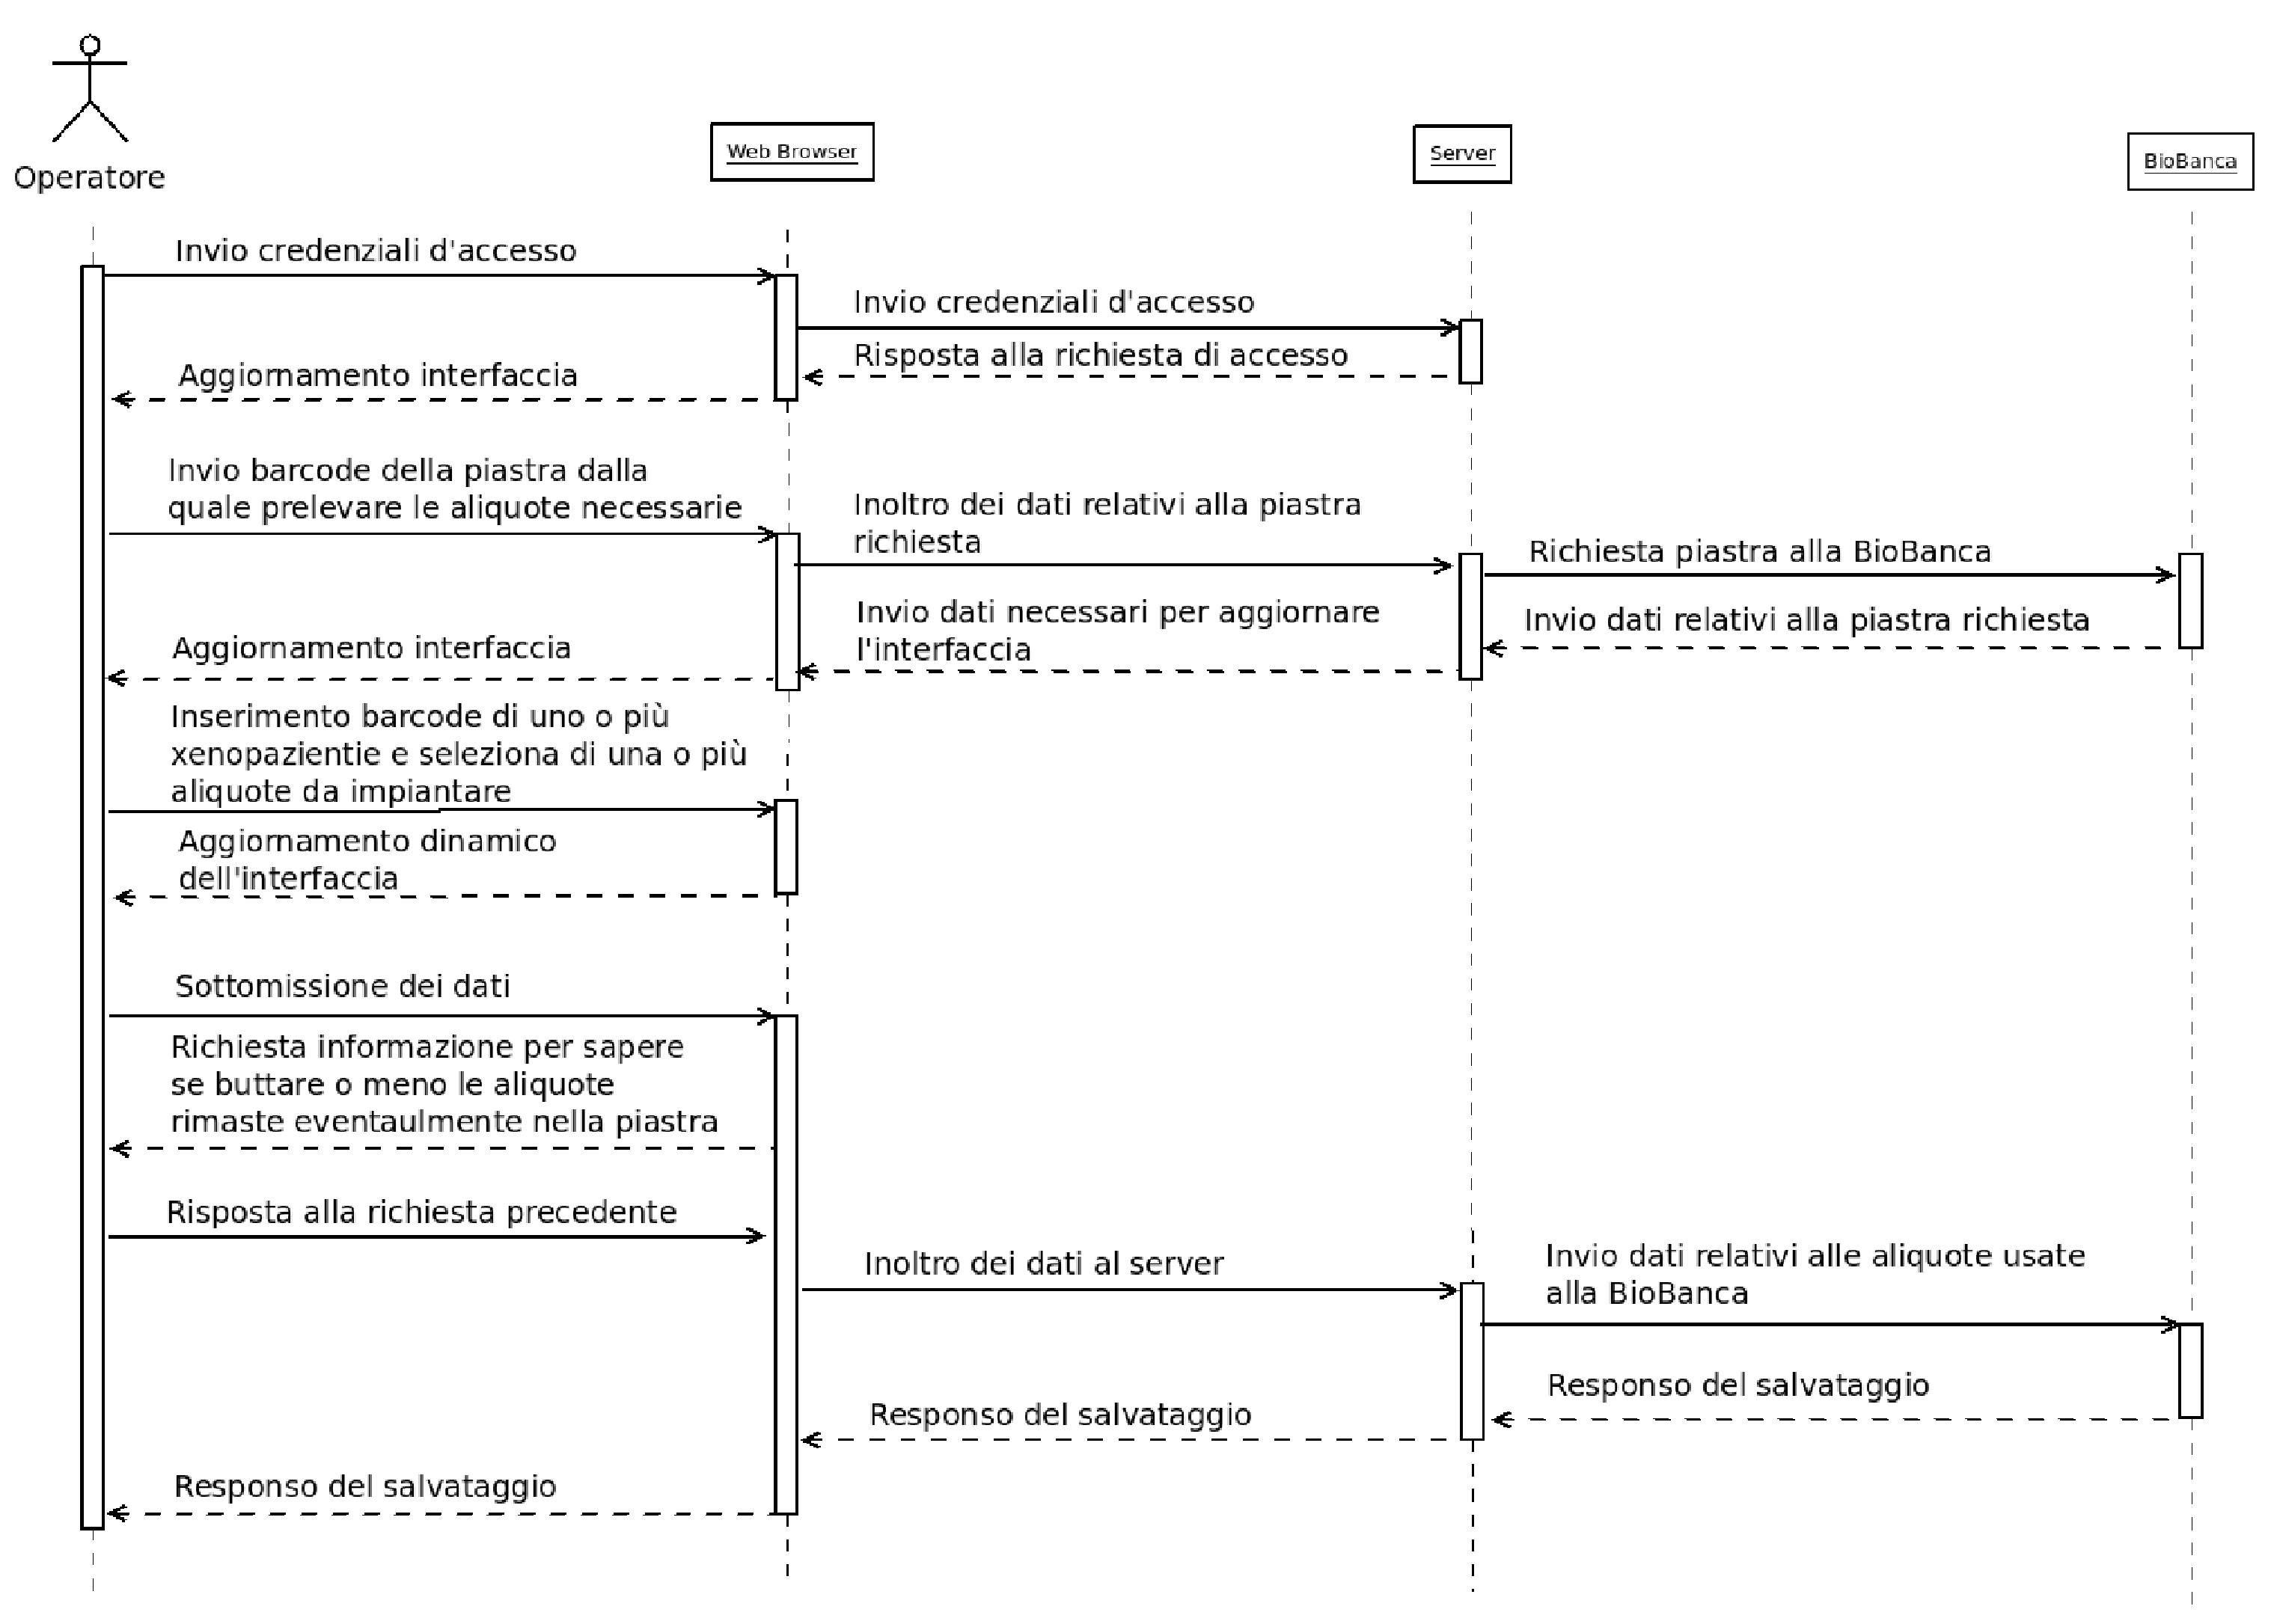
\includegraphics[width=0.9\textwidth]{./Figure/SDimplants}
\end{center}
\caption{Diagramma delle sequenze delle operazioni effettuate per creare un trattamento\label{fig:SDimpl}}
\end{figure}

\newpage

\section{Espianti}

Nel momento in cui si desidera effettuare una serie di espianti, per collezionare del materiale, si deve utilizzare una prima schermata preliminare, per selezionare i dati da elaborare nella pagina successiva. In questa prima interfaccia, si accede all'elenco degli \textit{xenopazienti} sui quali \`e stato programmato un espianto. Oltre a selezionare uno o pi\`u topi di questa lista, si devono anche selezionare i tipi di tessuto che si intendono generare durante l'espianto, in modo tale da poter gestire pi\`u efficacemente la schermata successiva. Un'ultimo parametro da introdurre \`e la data in cui viene effettuata questa operazione (la data di default \`e quella odierna). Questi dati preliminari consentono di inserire nel database le informazioni relative alla serie di espianti che si va a effettuare. In Figura~\ref{fig:UCDexpl} \`e riportato il diagramma dei casi d'uso relativo a questa interfaccia.

\begin{figure}[h]
\begin{center}
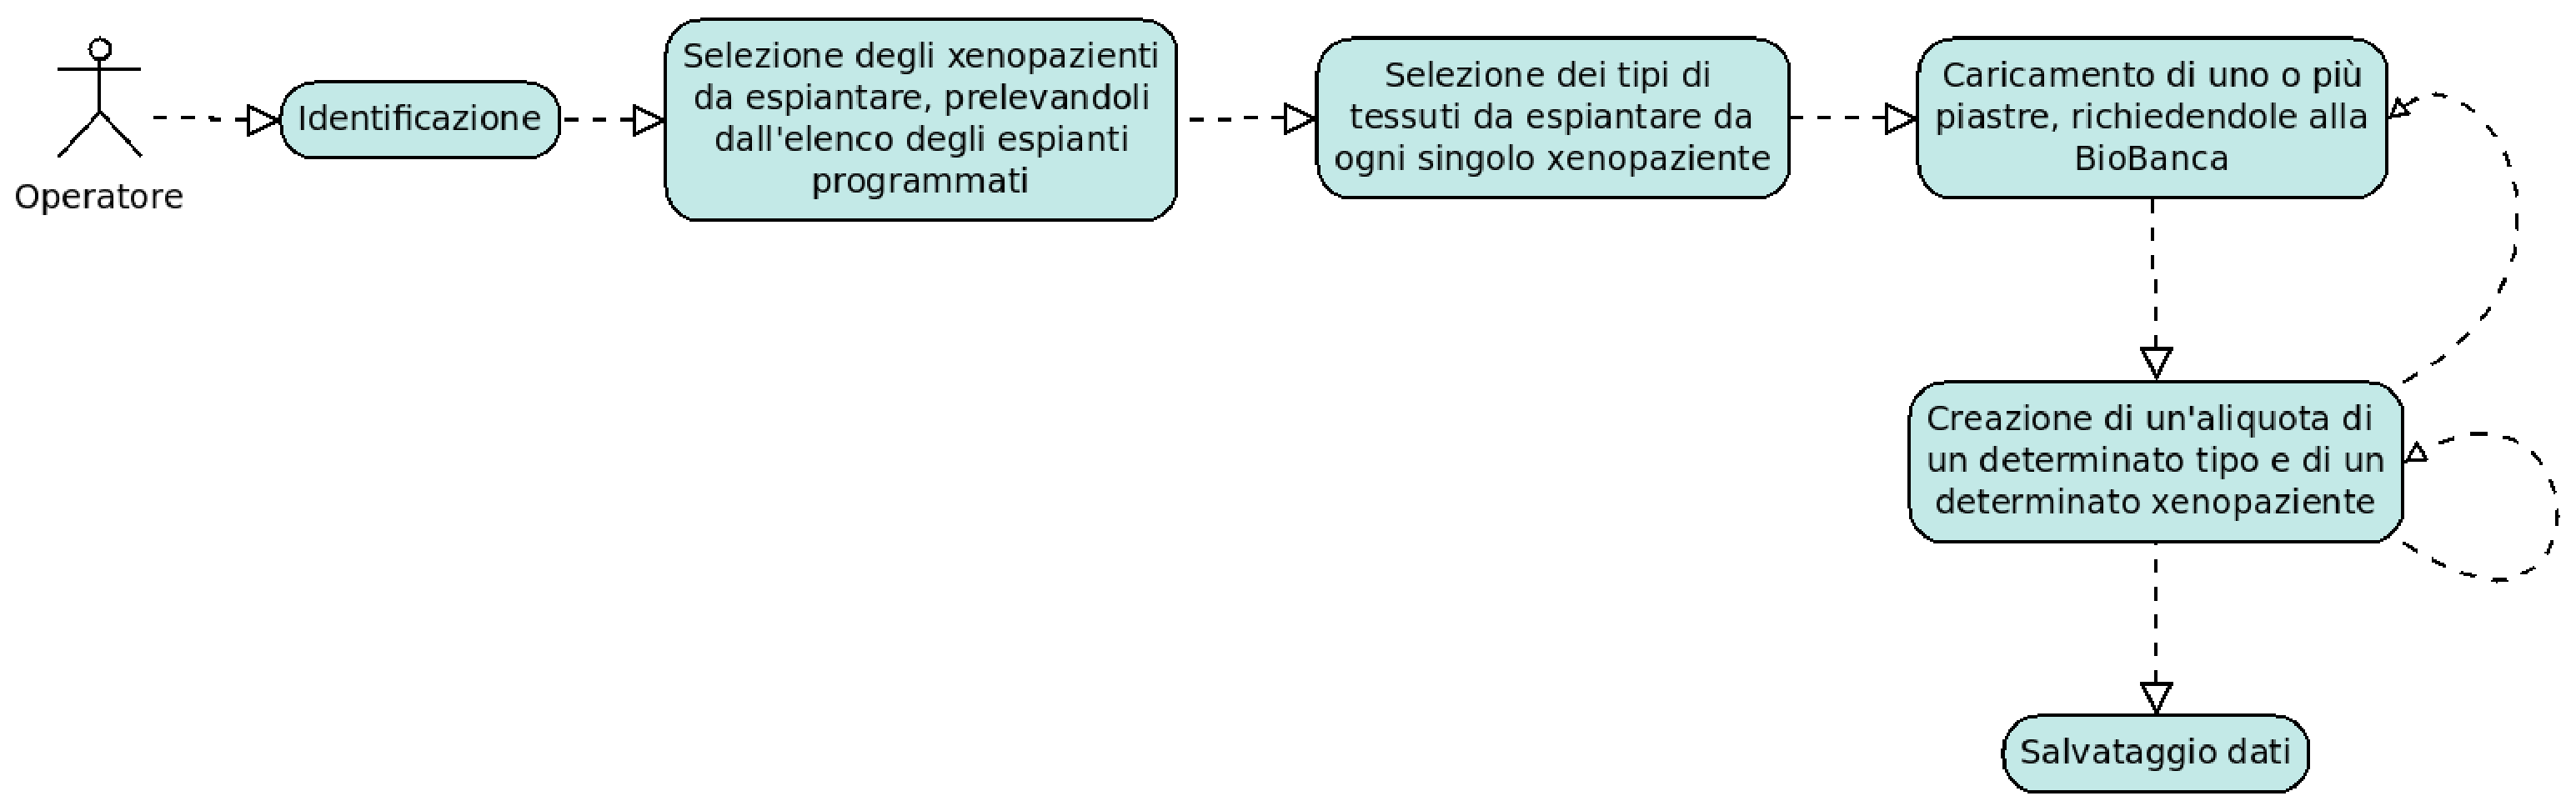
\includegraphics[width=0.8\textwidth]{./Figure/UCDexplants}
\end{center}
\caption{UCD relativo agli espianti\label{fig:UCDexpl}}
\end{figure}

Dopo aver visionato e selezionati gli xenoapazienti che si intendono espiantare, si accede ad un'interfaccia per gestire la collezione di nuovo materiale biologico. Questa schermata \`e stata costruita con l'intento di simulare l'ambiente di laboratorio. Questo rende agevole l'impatto con questa interfaccia agli addetti ai lavori, i quali conoscono bene le procedure di studio e ricerca.

Durante l'espianto, l'operatore pu\`o destinare le aliquote prelevate dal topo, in diversi tipi di provette, a loro volta contenute in diverse categorie di piastre (una piastra \`e un supporto in grado di contenere diverse provette al suo interno). Per simulare questa possibilit\`a di scelta, si \`e creata una tabella per ogni tipologia di piastra, dove ogni cella rappresenta una provetta in cui depositare il tessuto ottenuto dall'espianto appena eseguito. Le diverse piastre rispondono alla necessit\`a di avere diversi tipi di conservazione dei tessuti. Questa interfaccia, presentatata nella Figura~\ref{fig:explForm}, offre sei tabelle, ognuna rappresentante una diversa procedura per conservare il materiale:
\begin{itemize}
	\item \textbf{vital}: le aliquote vengono tenute un giorno in congelatore a -80\textcelsius\ e poi conservate in azoto liquido a -196\textcelsius;
	\item \textbf{snap frozen}: si effettua un rapido congelamento attraverso l'impiego di azoto liquido, per poi conservare le aliquote a -80\textcelsius;
	\item \textbf{RNAlater}: il tessuto \`e immerso in una soluzione acquosa per stabilizzare e proteggere i tessuti freschi, senza avere l'obbligo della conservazione in un congelatore (anche se cos\`i si aumenta il tempo per il quale l'aliquota pu\`o essere conservata). La soluzione acquosa \`e un fissativo blando e serve soprattutto per conservarre gli acidi nucleici. Vengono tenuti in frigo per 24h e poi congelati a -80\textcelsius;
	\item \textbf{formalin fixed}: i frammenti di tessuto vengono fissati per 24h in una soluzione contenente formalina e poi inclusi in un blocco di paraffina al fine di conservarli a temperatura ambiente (\`e il classico metodo di archiviazione utilizzato negli ospedali);
	\item \textbf{OCT frozen}: l'aliquota viene inglobata in una particolare resina chiamata OCT, che solidifica a basse temperature. Successivamente, si conserva in freezer, a -80\textcelsius;
	\item \textbf{ChinaBlack}: il tessuto viene insufflato con una soluzione di nero di china in modo da far risaltare eventuali metastasi come punti chiari su un fondo nero. Il materiale viene poi conservato a temperatura ambiente in una soluzione fissativa a base di metanolo e formaldeide. 
\end{itemize}

\begin{figure}[h]
\begin{center}
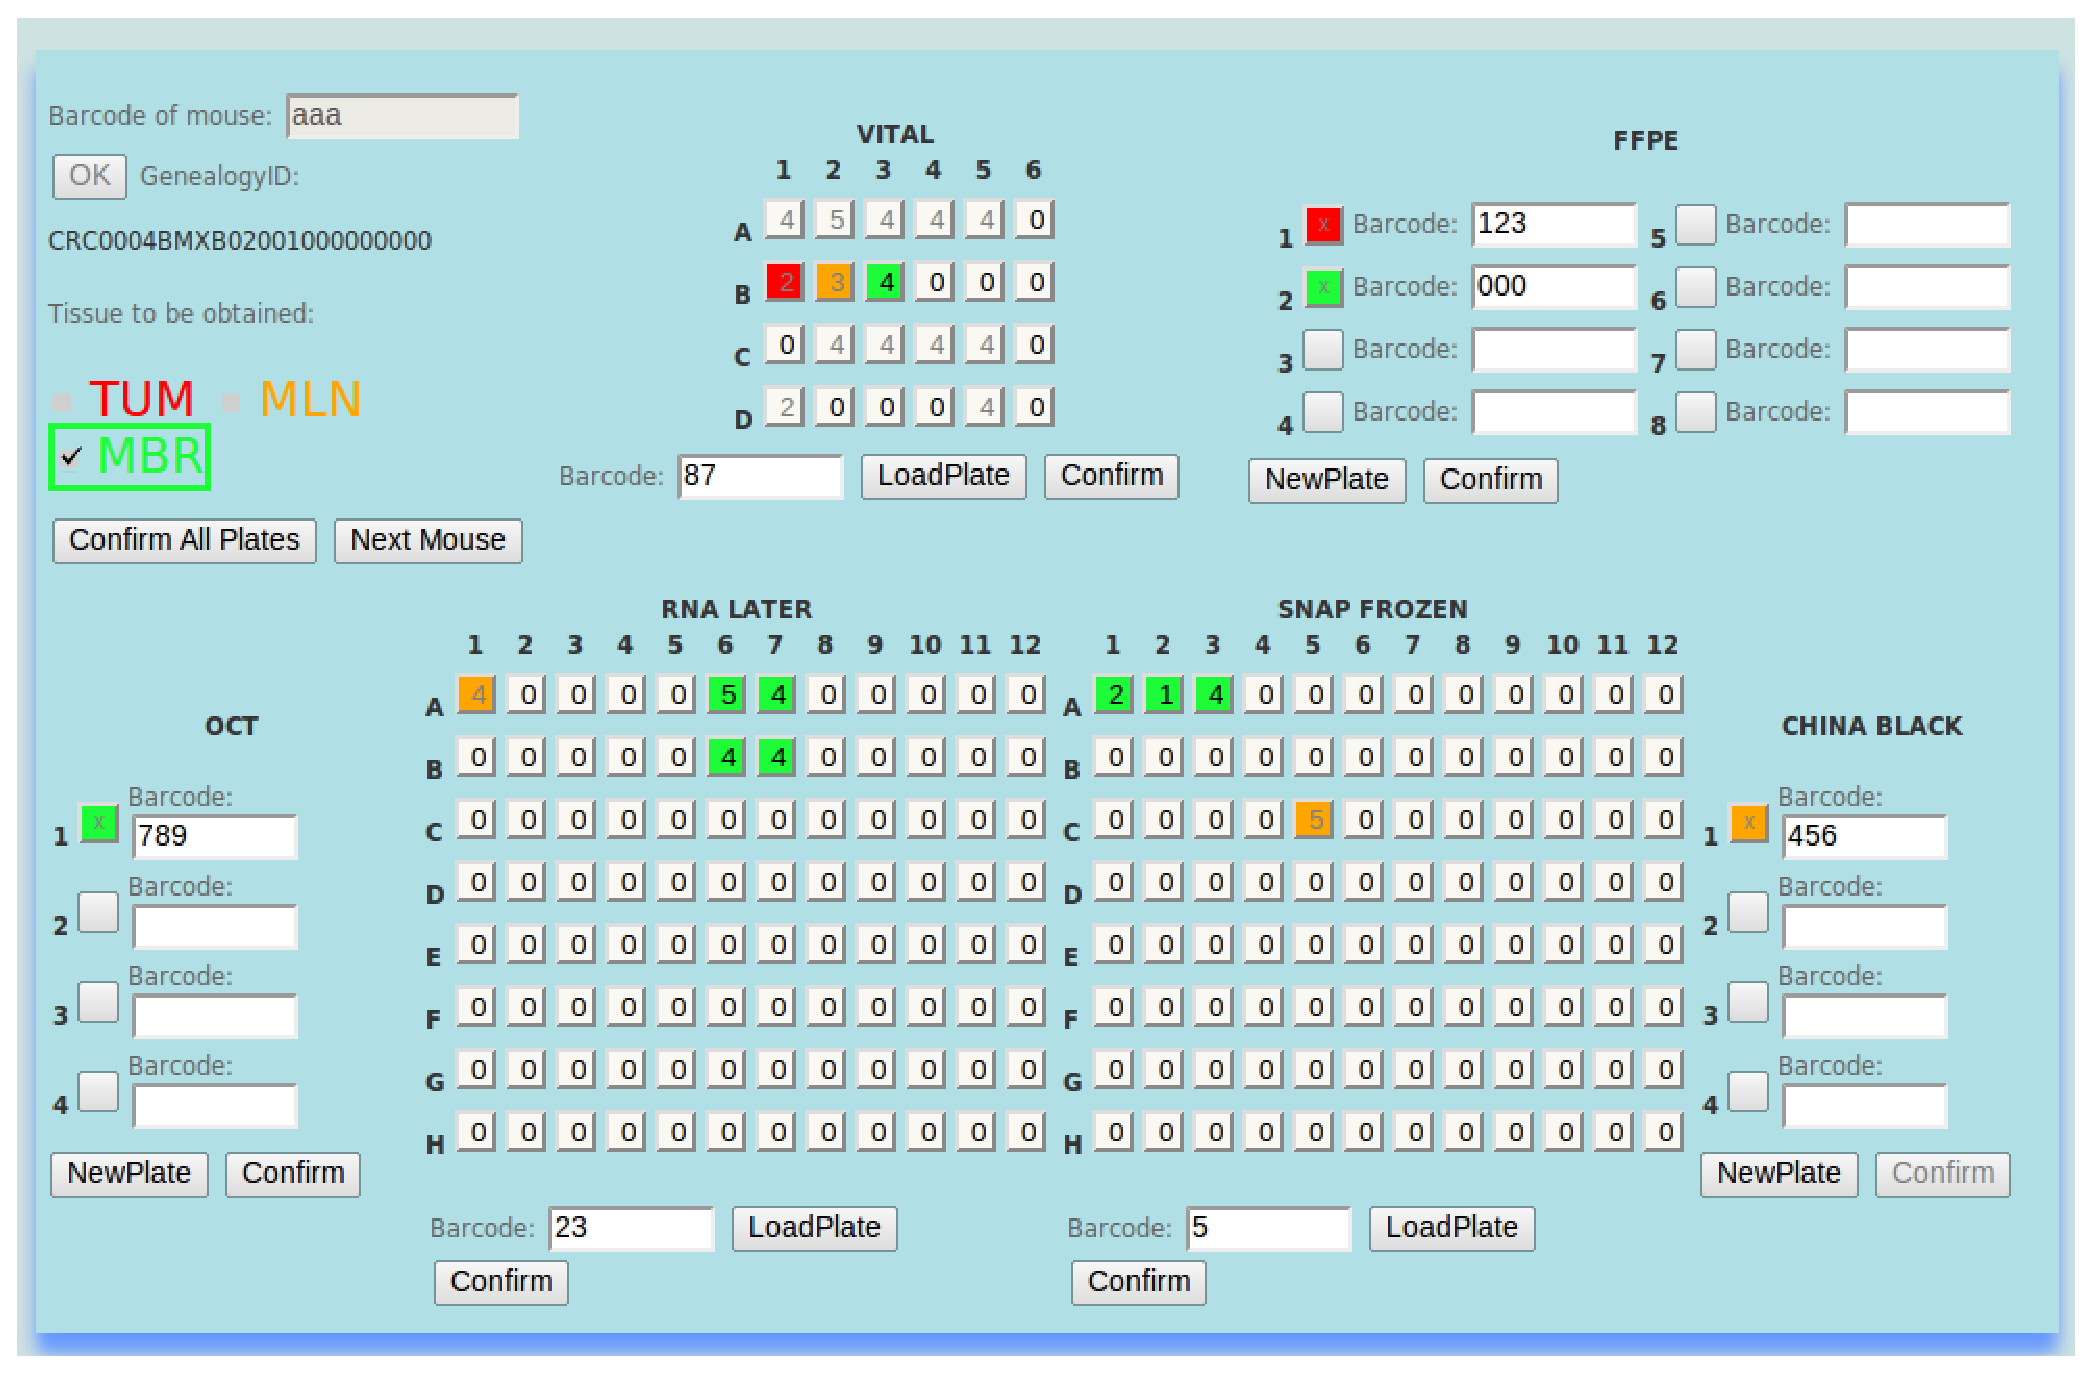
\includegraphics[width=1.0\textwidth]{./Figure/explantForm}
\end{center}
\caption{Struttura della pagina per collezionare i vari tessuti\label{fig:explForm}}
\end{figure}\newpage

L'operatore, per inserire le aliquote in queste tabelle, procede inserendo il barcode dello xenopaziente da espiantare. Successivamente, carica i dati delle piastre sulle quali vuole lavorare, inviandone cos\`i il barcode alla BioBanca. Dopodich\`e, inserisce i singoli tessuti nelle varie provette, a seconda del tipo di conservazione. In caso di errore, si pu\`o rimediare attraverso un'apposita lista, nella quale sono inserite le ultime operazioni effettuate. 

Una volta espiantati tutti i topi precedentemente selezionati, si procede con il salvataggio, articolato in pi\`u fasi. Si inviano i dati di tutte le aliquote create nella serie alla BioBanca, la quale tenta di salvarle nel proprio database. All'applicazione \Xeno\ arriva il responso sull'esito della transazione. In caso positivo, XMS avvia a sua volta il salvataggio dei dati. L'esito di questa operazione \`e notificata alla BioBanca, che, in caso negativo, effettua il rollback sulle informazioni precedentemente salvate. Infine, a seconda degli esiti delle precedenti operazioni, si visualizza il report dei dati creati o un messaggio d'errore. Questo flusso logico di dati \`e descritto in Figura~\ref{fig:flussoExpl}, mentre in Figura~\ref{fig:SDexpl} si pu\`o osservare il diagramma delle sequenze di questa interfaccia.


\begin{figure}[h]
\begin{center}
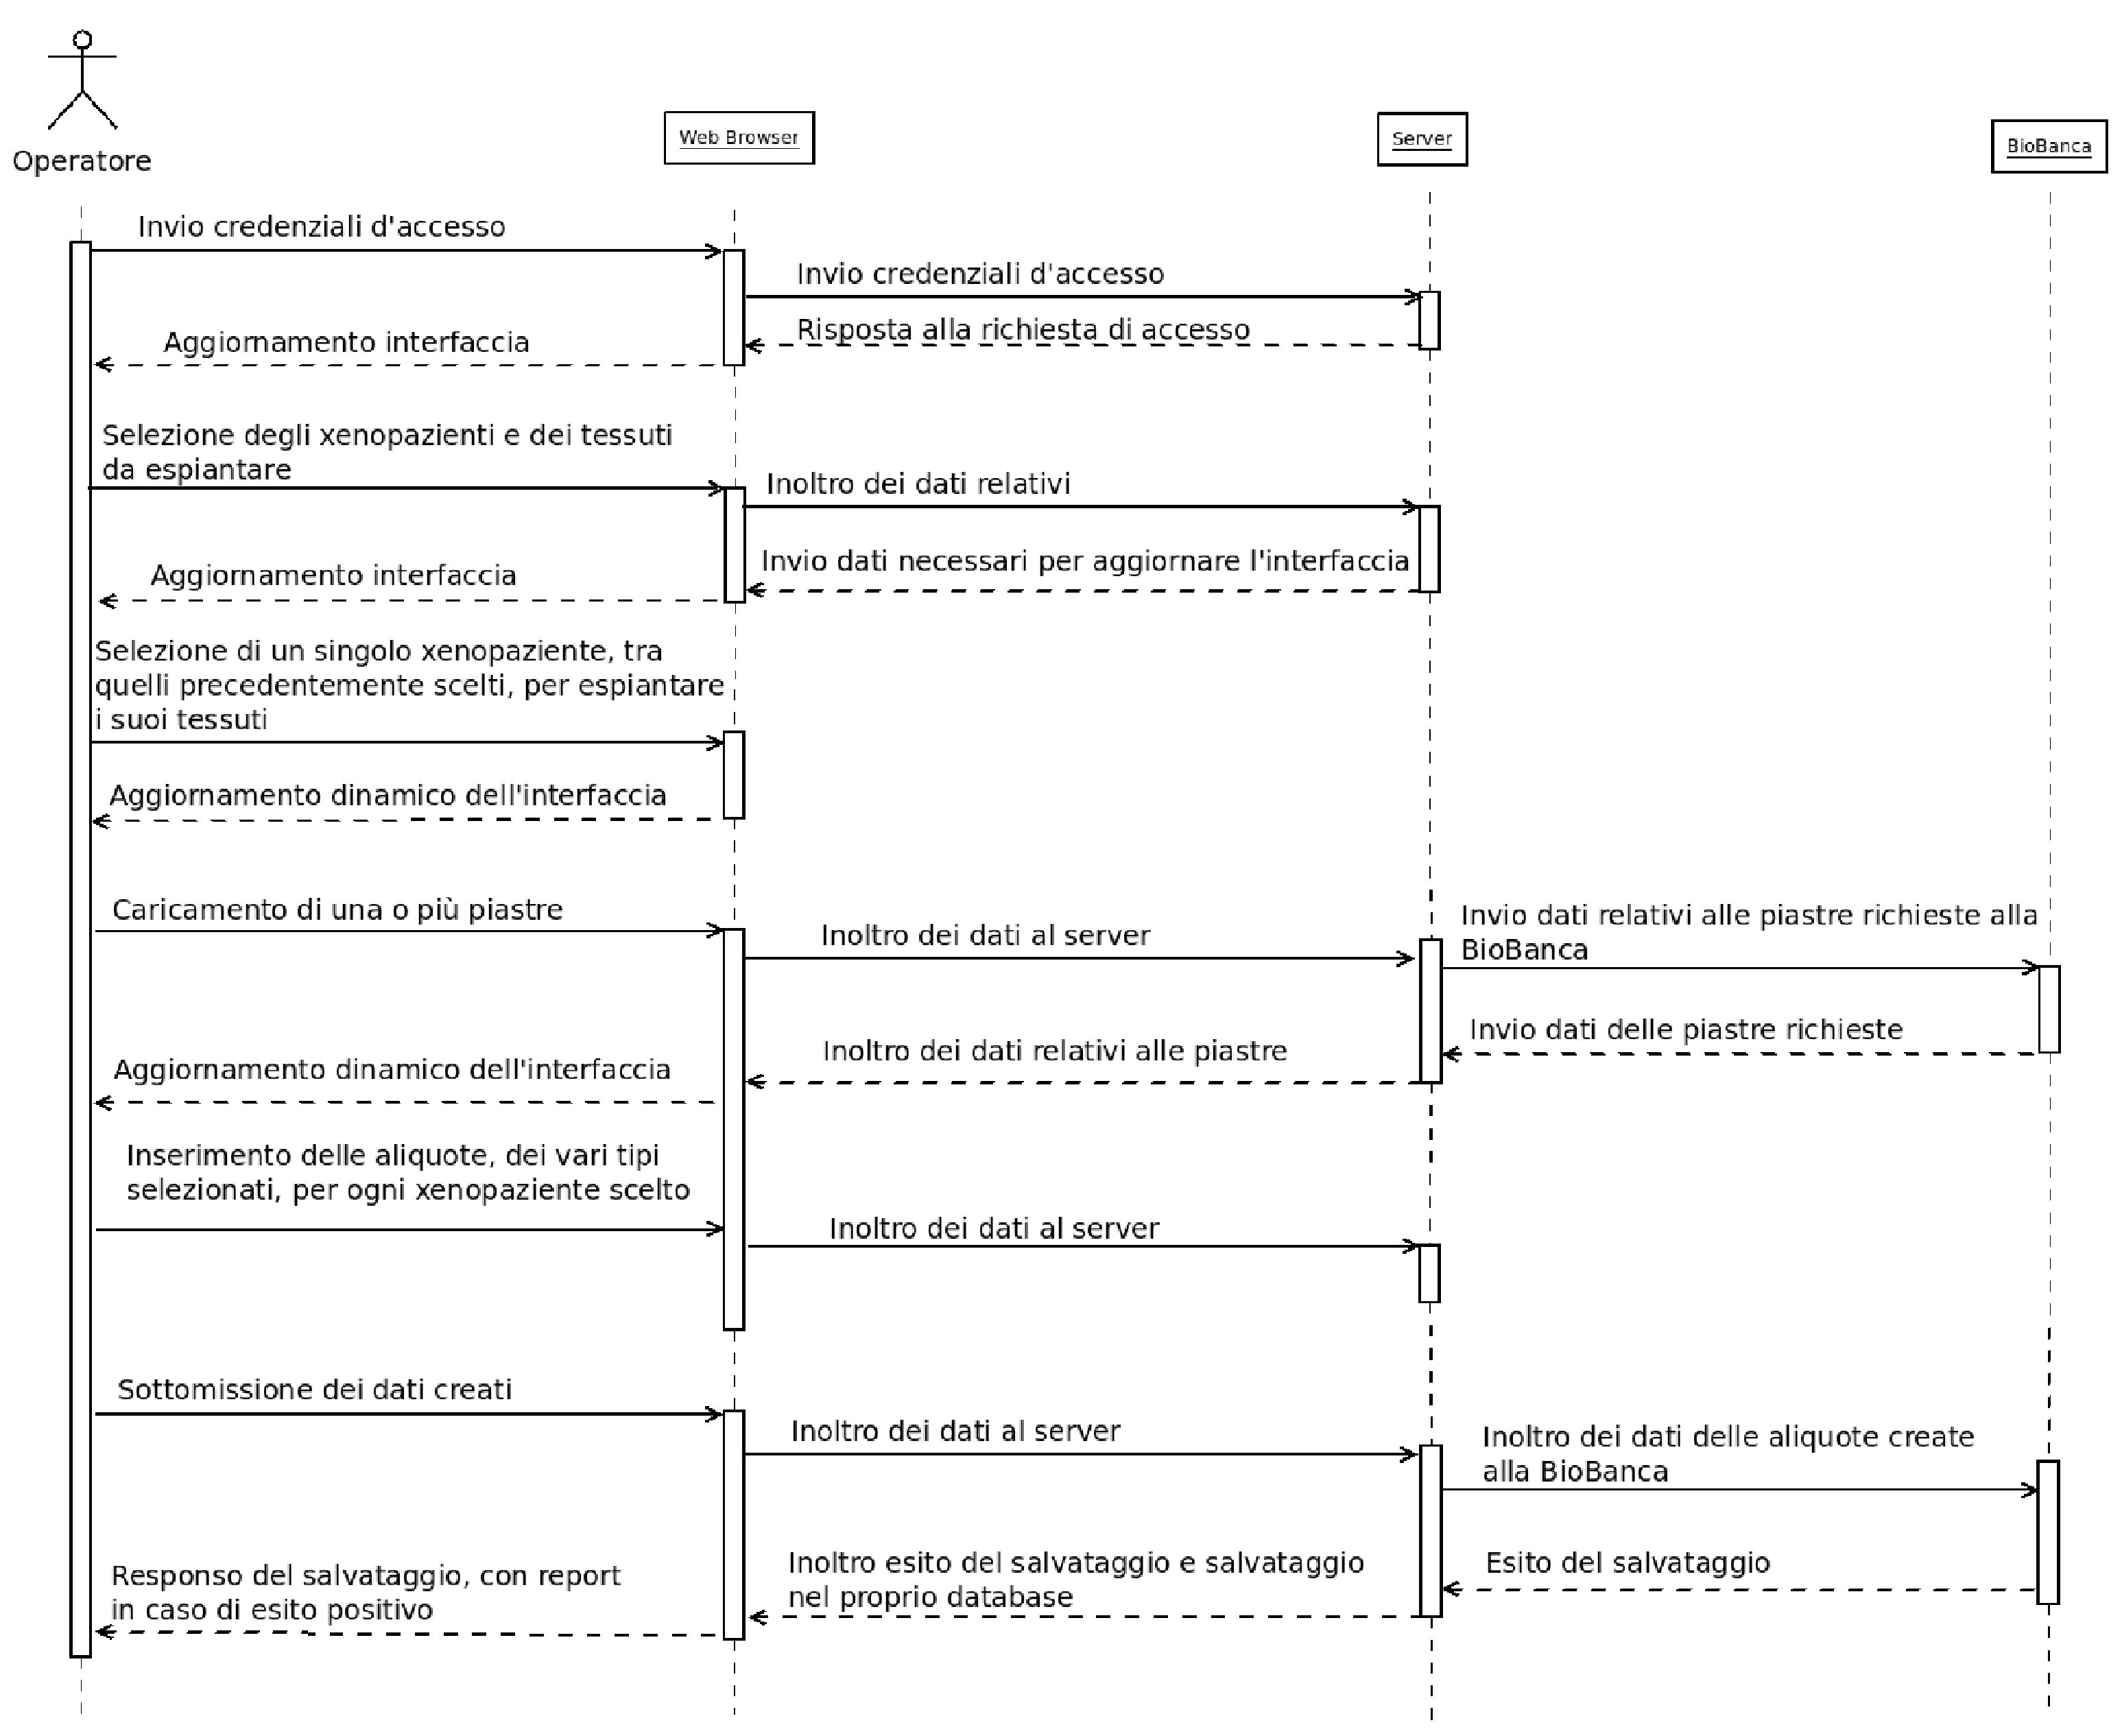
\includegraphics[width=0.9\textwidth]{./Figure/SDexplants}
\end{center}
\caption{Diagramma delle sequenze relativo agli espianti\label{fig:SDexpl}}
\end{figure}

\begin{figure}[h]
\begin{center}
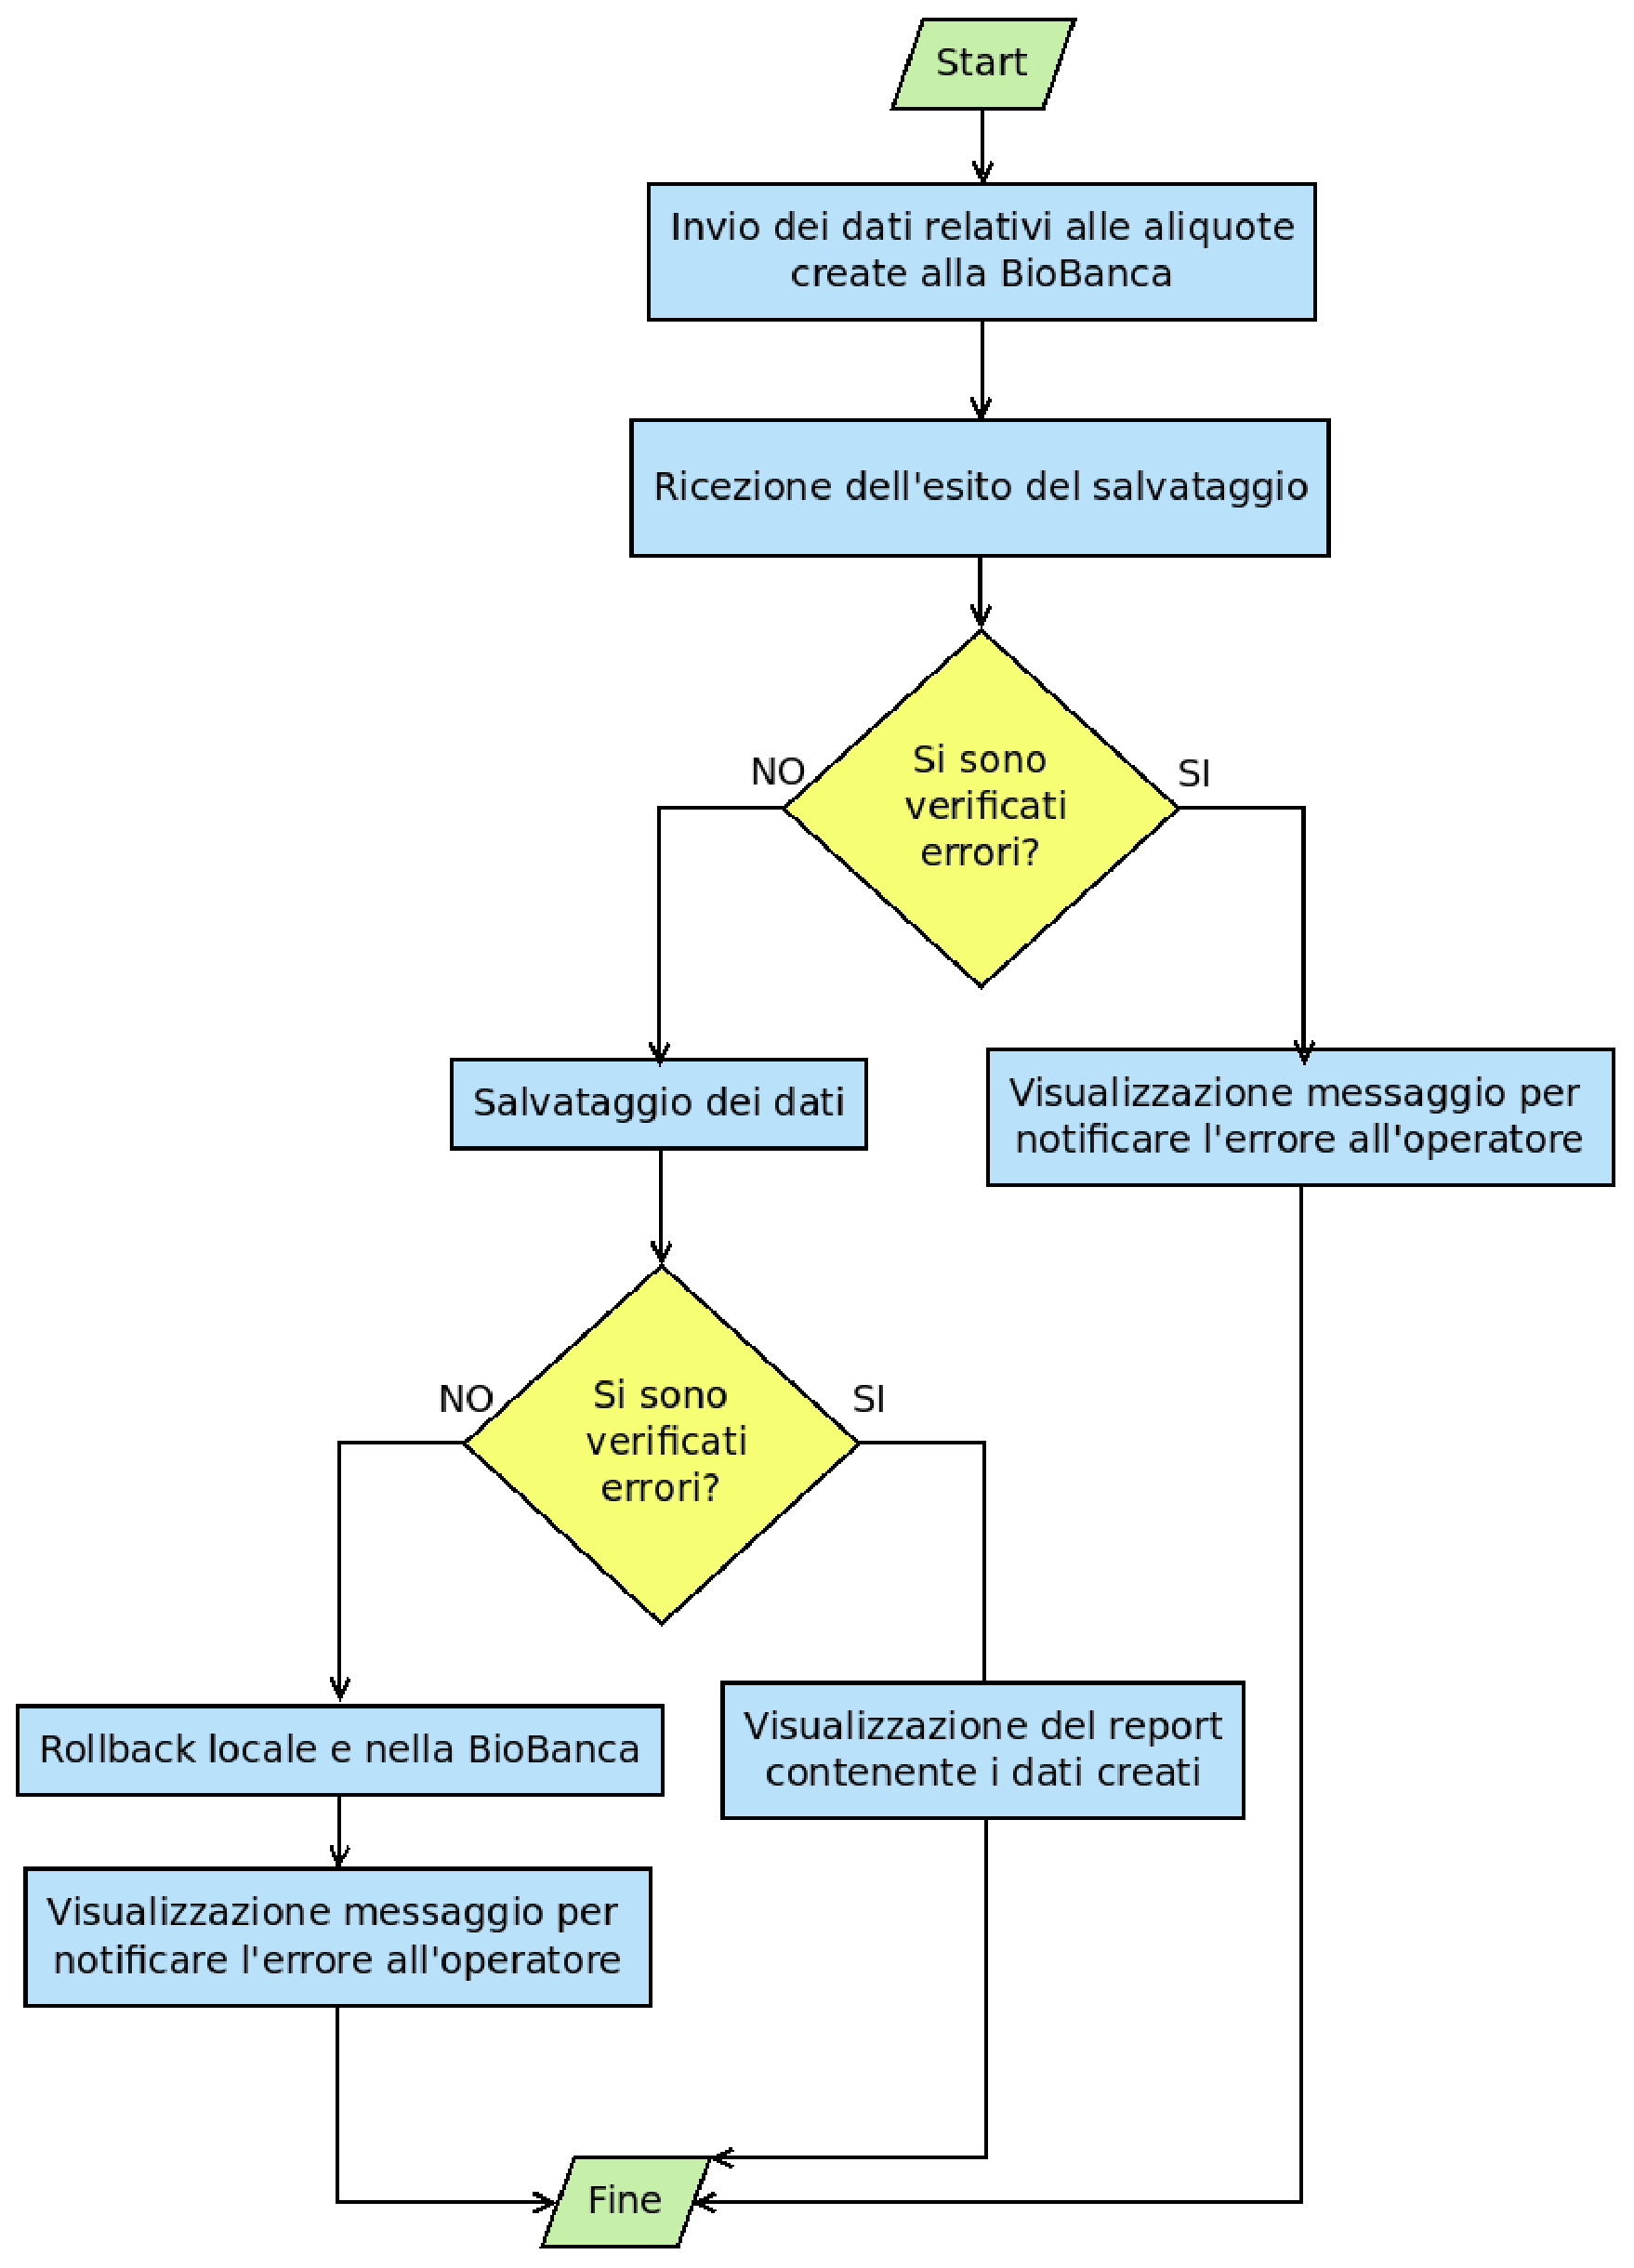
\includegraphics[width=0.8\textwidth]{./Figure/flussoExplants}
\end{center}
\caption{Diagramma di flusso delle comunicazione con la BioBanca\label{fig:flussoExpl}}
\end{figure}
